%!TEX program = xelatex
\documentclass[aspectratio=169,UTF8,11pt]{ctexbeamer}

    \mode<presentation> {
    \usetheme{Madrid}
    %\setbeamertemplate{footline} % To remove the footer line in all slides uncomment this line
    \setbeamertemplate{footline}[frame number] % To replace the footer line in all slides with a simple slide count uncomment this line
    \setbeamercolor{page number in head/foot}{fg=blue}
    \setbeamertemplate{navigation symbols}{} % To remove the navigation symbols from the bottom of all slides uncomment this line
    }
    \usepackage{indentfirst}
    \setlength{\parindent}{2em}
    \usepackage{listings}
    \usepackage{wrapfig}
    \usepackage{graphicx}
    % \usepackage{fboxrule}

    \definecolor{indiagreen}{rgb}{0.07, 0.53, 0.03}
    \definecolor{indianred}{rgb}{0.8, 0.36, 0.36}
    \definecolor{indianyellow}{rgb}{0.89, 0.66, 0.34}
    \definecolor{bondiblue}{rgb}{0.0, 0.58, 0.71}
    \definecolor{ao(english)}{rgb}{0.0, 0.5, 0.0}
    \definecolor{azure(colorwheel)}{rgb}{0.0, 0.5, 1.0}
    \definecolor{alizarin}{rgb}{0.82, 0.1, 0.26}
    % User Defined Block %%%%%%%%%%%%%%%%%%%%%%%%%%%%%%%%%%%%%%%%%%%%%%%%%%%%%%%%
    \newenvironment<>{abstractblock}[1]{%
      \setbeamercolor{block title}{fg=white,bg=bondiblue}%
    %   \setbeamercolor{block body}{fg=white,bg=bondiblue}%
      \begin{block}#2{#1}}{\end{block}}

    \newenvironment<>{adviceblock}[1]{%
    % \setbeamercolor{block title}{fg=white,bg=bondiblue}%
      \setbeamercolor{block body}{fg=white,bg=alizarin}%
    \begin{block}#2{#1}}{\end{block}}

    \newenvironment<>{thinkblock}[1]{%
      \setbeamercolor{block title}{fg=white,bg=azure(colorwheel)}%
    %   \setbeamercolor{block body}{fg=white,bg=bondiblue}%
      \begin{block}#2{#1}}{\end{block}}

    \newenvironment<>{yellowblock}[1]{%
      \setbeamercolor{block title}{fg=white,bg=indianyellow}%
      \begin{block}#2{#1}}{\end{block}}

    \lstset{language=C++,
    columns=flexible,
    basicstyle=\footnotesize\ttfamily,                                    % 设定代码字体、大小
    %numbers=left,xleftmargin=2em,framexleftmargin=2em,                   % 在左侧显示行号
    %numberstyle=\color{darkgray},                                        % 设定行号格式
    keywordstyle=\color{blue},                                            % 设定关键字格式
    commentstyle=\color{ao(english)},                                     % 设置代码注释的格式
    stringstyle=\color{brown},                                            % 设置字符串格式
    showstringspaces=false,                                              % 控制是否显示空格
    %frame=single,                                                         % 控制外框
    breaklines,                                                           % 控制是否折行
    % postbreak=\space,                                                     % 控制折行后显示的标识字符
    breakindent=5pt,                                                      % 控制折行后缩进数量
    emph={size\_t,array,deque,list,map,queue,set,stack,vector,string,pair,tuple,ostream}, % 非内置类型
    emphstyle={\color{teal}},
    escapeinside={(*@}{@*)},
}


    \title
        [第3章~语句控制结构\hspace{2em}]
        {第3章~语句控制结构}

%\author[李长河]{李长河} % Your name
%\institute[CUG] % Your institution as it will appear on the bottom of every slide, may be shorthand to save space
%{
%中国地质大学(武汉)\\ % Your institution for the title page
%\medskip
%\textit{lichanghe@cug.edu.cn} % Your email address
%}
\date{} % Date, can be changed to a custom date


\begin{document}

\maketitle

\section{语句}
\subsection{空语句}
\subsection{复合语句}
\subsection{控制语句作用域}


\section{分支结构}
\subsection{\texttt{if}语句}
\subsection{\texttt{switch}语句}

\section{循环结构}
\subsection{\texttt{while}语句}
\subsection{\texttt{do while}语句}
\subsection{\texttt{for}语句}

\section{跳转语句}
\subsection{\texttt{break}语句}
\subsection{\texttt{continue}语句}

\section{嵌套结构和应用实例}

\begin{frame}
	{目录}
	\tableofcontents
\end{frame}

\begin{frame} {~~}
	\begin{yellowblock}{学习目标}
		\begin{itemize}
			\item 掌握基本语句控制结构的语法和特点;
			\item 学会运用基本控制结构解决简单问题;
			\item 理解并能够运用\alert{递推法}和\alert{穷举法}解决实际应用问题。
		\end{itemize}
	\end{yellowblock}
\end{frame}

\begin{frame}
	{3.1 语句\small{—空语句}}
	\begin{block}{语句}
		表达式后面加上分号就变成了一个表达式语句(\texttt{expression statement})。\\
		如:\\
		\setlength\parindent{2em}
		\indent\indent \alert{\texttt{counter + 1;}}~~~~//一条没有实际意义的表达式语句\\
		\indent\indent \texttt{counter += 1;}~~//一条有用的复合赋值语句\\
	\end{block}

	\begin{block}{空语句}
		\begin{itemize}
			\item 只有一个分号构成的语句,如:\\
			      \setlength\parindent{2em}
			      \texttt{;}~~~~//空语句\\
			\item 空语句不会执行任何操作,如:\\
			      \texttt{counter += 1;;}~~~~//第二个分号不会影响该语句的执行\\
		\end{itemize}
	\end{block}



	\begin{columns}
		\begin{column}{0.1\textwidth}
			% \setbeamercolor{bgcolor}{fg=black,bg=brown!80!yellow}
			\begin{beamercolorbox}[rounded=true, shadow=false,wd=0pt]{bgcolor}
				
\includegraphics[scale=0.6]{question_fig.jpg}
			\end{beamercolorbox}
		\end{column}

		\begin{column}{0.9\textwidth}
			\setbeamercolor{bgcolor}{fg=black,bg=green!50!white}
			\begin{beamercolorbox}[rounded=true, shadow=false,wd=4cm]{bgcolor}
				是否可以随意使用分号?
			\end{beamercolorbox}
		\end{column}
	\end{columns}

\end{frame}

\begin{frame}[fragile]
	{3.1 语句\small{—复合语句}}
	\begin{block}{复合语句}
		\begin{itemize}
			\item \alert{复合语句}(\texttt{compound statement})指用\alert{花括号}括起来的语句和声明序列,也被称作\alert{语句块}。\\
			\item 在块内引入的名字只在块内可见,如:\\
			      \begin{lstlisting}[basicstyle=\small\ttfamily]
            { //语句块开始
                int sum = 0; // 定义一个对象
                /*...*/
            } //语句块结束
            \end{lstlisting}
		\end{itemize}
	\end{block}
\end{frame}

\begin{frame}[fragile]
	{3.1 语句\small{—控制结构语句作用域}}
	\begin{block}{\texttt{C++}控制结构语句包括:}
		\begin{itemize}
			\item \textcolor[rgb]{0,0,1}{\texttt{if}}语句
			\item \textcolor[rgb]{0,0,1}{\texttt{switch}}语句
			\item \textcolor[rgb]{0,0,1}{\texttt{while}}语句
			\item \textcolor[rgb]{0,0,1}{\texttt{for}}语句
		\end{itemize}
	\end{block}
\begin{yellowblock}<2->{控制结构语句作用域}
这些控制语句的作用域\alert{只包括紧跟其后的一条语句}
\end{yellowblock}
\end{frame}

\begin{frame}[fragile]
	{3.1 语句\small{—控制结构语句作用域}}
	\begin{exampleblock}{下面\texttt{while}语句的作用域是什么?}
		\begin{lstlisting}[basicstyle=\small\ttfamily]
            while(counter < 10 )
                ++counter;
           sum += counter;
            \end{lstlisting}
	\end{exampleblock}
	\begin{block}{可用花括号扩展其作用域,如:}
		\begin{lstlisting}[basicstyle=\small\ttfamily]
            while(counter < 10 ){  //while作用域从这里开始
                ++counter;
                sum += counter;
            }  //while作用域到这里结束
            \end{lstlisting}
	\end{block}
\end{frame}


\begin{frame}[fragile]
	\frametitle{3.2 分支结构}
	\begin{abstractblock}{\texttt{C++}提供了两种分支形式}
		\begin{itemize}
			\item \textcolor[rgb]{0,0,1}{\texttt{if}} 语句
			\item \textcolor[rgb]{0,0,1}{\texttt{switch}} 语句
		\end{itemize}
	\end{abstractblock}
\end{frame}

\begin{frame}[fragile]
	\frametitle{3.2 分支结构\small{—\texttt{if}语句}}
	% \framesubtitle{——\texttt{if}语句}
	\begin{columns}
		\begin{column}{0.48\textwidth}
			\begin{block}<1->{\texttt{if}语句的语法格式:}
				\begin{lstlisting}[basicstyle=\small\ttfamily]
if (expr) {         //条件表达式
    statement;      //语句
}
        \end{lstlisting}
			\end{block}
			\begin{block}<2->{\texttt{else}分支结构格式:}
				\begin{lstlisting}[basicstyle=\small\ttfamily]
if (expr) {
    statement1;  //分支语句1
}
else {
    statement2;  //分支语句2
}
     \end{lstlisting}
				\alert{建议}:尽量使用花括号改善程序的可读性
			\end{block}
		\end{column}
		\begin{column}<2->{0.48\textwidth}
			\begin{figure}[ht]
				\centering
				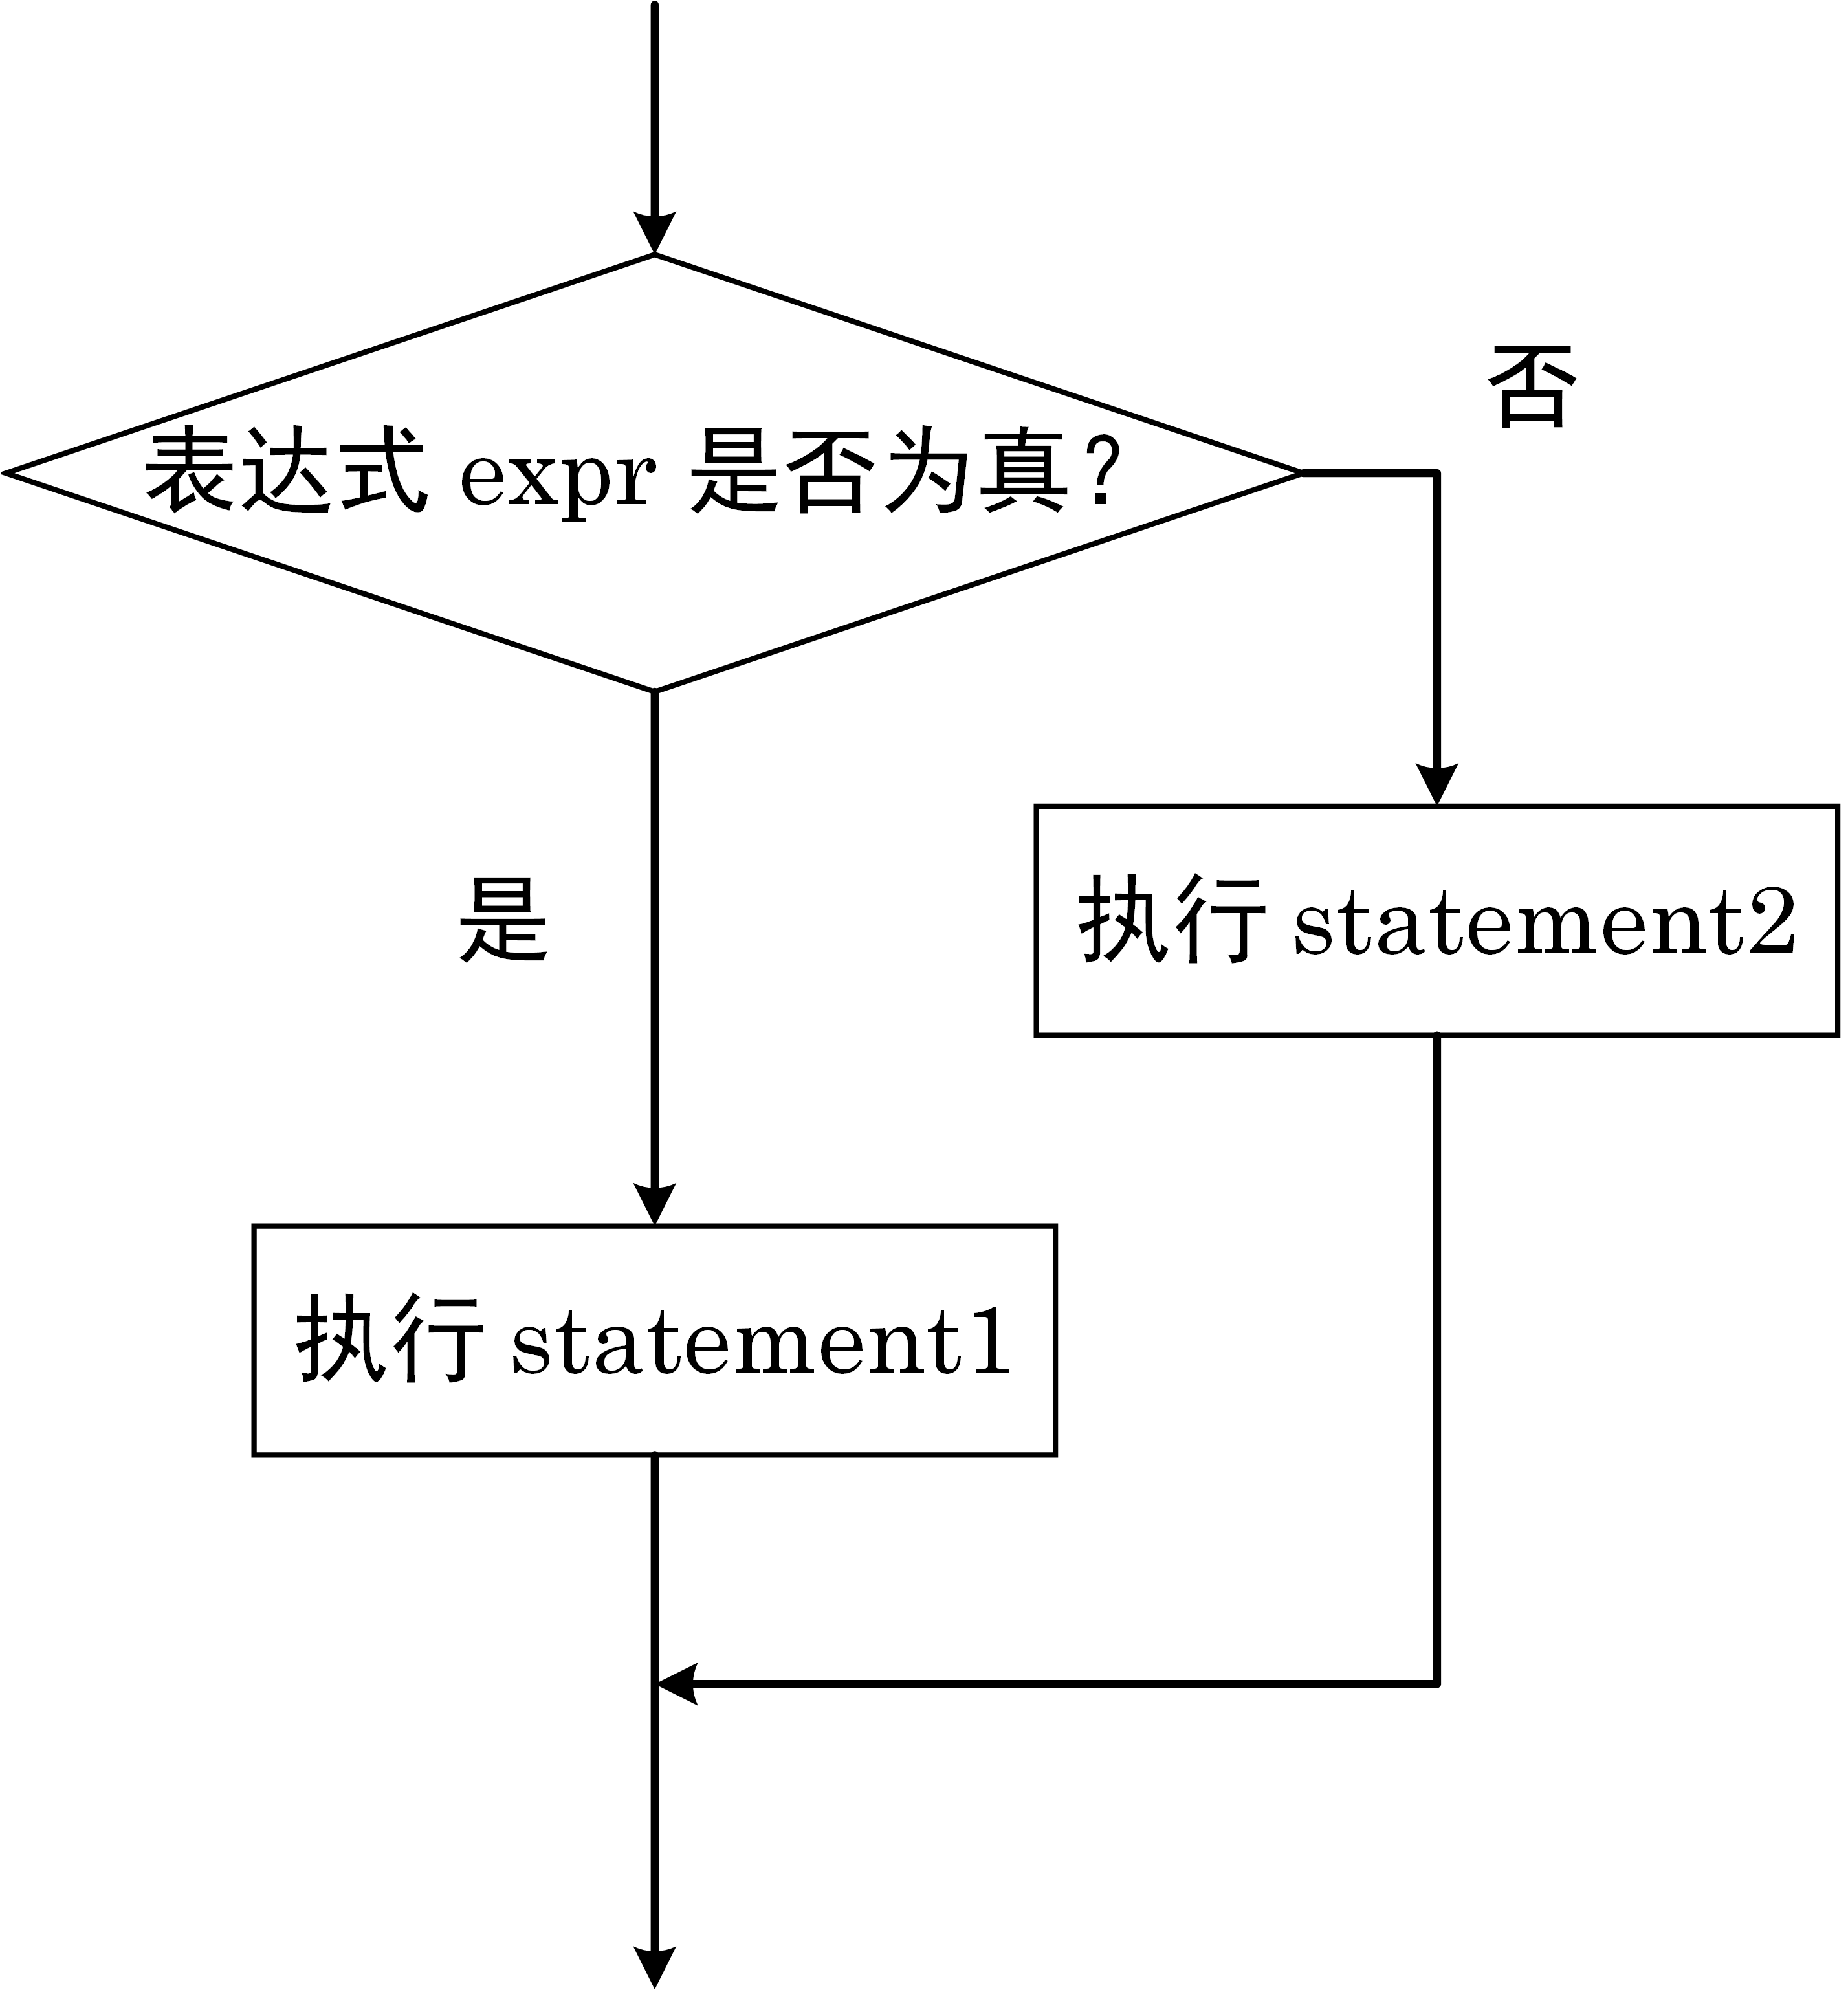
\includegraphics[scale=0.5]{IF_statement.png}
				% \caption{\texttt{else}分支结构执行流程}
				% \label{fig:label}
			\end{figure}
		\end{column}
	\end{columns}
\end{frame}


\begin{frame}[fragile]
	\frametitle{3.2 分支结构\small{—\texttt{if}语句}}
	\begin{exampleblock}{练习:找出下面程序段中的错误}
		\begin{columns}
			\begin{column}[t]{0.48\textwidth}
				\begin{lstlisting}[basicstyle=\small\ttfamily]
    1. if (val1 != val2)
           val1 = val2
       else
           val1 = val2 = 0;
        \end{lstlisting}
				\begin{lstlisting}[basicstyle=\small\ttfamily]
    3. if (val1 < val2)
        //执行以下两个语句
            val1 = 1;
            val2 = 2;
        \end{lstlisting}
			\end{column}
			\begin{column}[t]{0.48\textwidth}
				\begin{lstlisting}[basicstyle=\small\ttfamily]
    2. if (val1 = 10)
        //如果val等于10
            value = 1;
            \end{lstlisting}
				~\\
				\begin{lstlisting}[basicstyle=\small\ttfamily]
    4. if val1 < val2
        cin >> val1 >> endl;
            \end{lstlisting}
			\end{column}
		\end{columns}
	\end{exampleblock}
\end{frame}

\begin{frame}
	\frametitle{3.2 分支结构\small{—\texttt{if}语句}}
	% \framesubtitle{——\texttt{if}语句}
	\begin{exampleblock}{例3.1:}
		\ttfamily 判断一个整数是否大于0且是3的倍数。\\
	\end{exampleblock}
\end{frame}

\begin{frame}[fragile]
	\frametitle{3.2 分支结构\small{—\texttt{if}语句}}
	% \framesubtitle{——\texttt{if}语句}
	\begin{exampleblock}{代码清单3.1,例3.1:}
\vspace{-3mm}
		\begin{columns}
			\begin{column}{0.45\linewidth}
\begin{lstlisting}[numbers=left,numberstyle=\small,basicstyle=\normalsize\ttfamily]
#include<iostream>
using namespace std;
int main() {
    int n;
    cout << "请输入一个整数n:";
    cin >> n;
            \end{lstlisting}\ttfamily
			\end{column}
			\begin{column}{0.4\linewidth}
				\begin{lstlisting}[firstnumber=6,numbers=left,numberstyle=\small,basicstyle=\normalsize\ttfamily]
    //n大于0且被3整除
    if (n > 0 && n % 3 == 0) {
        cout << "Yes" << endl;
    }
    else {
        cout << "No" << endl;
    }
}
            \end{lstlisting}\ttfamily
			\end{column}
		\end{columns}
		\ttfamily 示例:输入:7~~输出:\texttt{No}~~~~输入:9~~输出:\texttt{Yes}
	\end{exampleblock}
\end{frame}

\begin{frame}
	\frametitle{3.2 分支结构\small{—\texttt{if}语句}}
	% \framesubtitle{——\texttt{if}语句}
	\begin{block}{嵌套的\texttt{if}语句}
		\begin{itemize}
			\item 有\alert{两个以上分支}时,选用\alert{嵌套的~\texttt{if}~ 语句结构}
			\item 内嵌~\texttt{if}语句既可以嵌套在~\texttt{if}~语句中,也可以嵌套在~\texttt{else}~语句中\\
		\end{itemize}
	\end{block}
	\begin{exampleblock}{例3.2:}
		\ttfamily 将百分制的成绩转换成五级制,如果成绩在90分到100分范围内(包括90分和100分),则转换成~\texttt{A}~,80分到90分为~ \texttt{B}~ (包括80分不包括90分),依次类推,60分以下为~\texttt{F}。
	\end{exampleblock}
\end{frame}

\begin{frame}[fragile]
	\frametitle{3.2 分支结构\small{—\texttt{if}语句}}
	% \framesubtitle{——\texttt{if}语句}
	\begin{exampleblock}{代码清单3.2,例3.2:}
		\begin{columns}[t]
			\begin{column}{0.06\textwidth}
			\end{column}
			\begin{column}{0.45\textwidth}
				\begin{lstlisting}[numbers=left,numberstyle=\small,basicstyle=\small\ttfamily]
#include<iostream>
using namespace std;
int main() {
    unsigned score;
    cout << "请输入一个分数:";
    cin >> score;
    if (score < 60) {
        cout << "F" << endl;
    }
    else if (score < 70) {
        cout << "D" << endl;
    }
        \end{lstlisting}\ttfamily
			\end{column}
			\begin{column}{0.09\textwidth}
			\end{column}
			\begin{column}{0.4\textwidth}
				\begin{lstlisting}[numbers=left,numberstyle=\small,firstnumber=13,basicstyle=\small\ttfamily]
    else if (score < 80) {
        cout << "C" << endl;
    }
    else if (score < 90) {
        cout << "B" << endl;
    }
    else {
        cout << "A" << endl;
    }
    return 0;
}
        \end{lstlisting}\ttfamily
			\end{column}
		\end{columns}
		\texttt{示例:输入76~~输出:C}
	\end{exampleblock}
\end{frame}


\begin{frame}[fragile]
	\frametitle{3.2 分支结构\small{—\texttt{if}语句}}
	% \framesubtitle{——\texttt{if}语句}
	\begin{block}{避免悬垂\texttt{else}}
		\begin{itemize}
			\item 上例中~\texttt{if}~和~\texttt{else}~语句个数相同,若~\texttt{if}~语句数目多于~\texttt{else}~语句数目,就会出现~\texttt{else}~和~\texttt{if}~匹配的问题,也称\alert{悬垂~\texttt{else(dangling else)}}。
			\item \texttt{C++}规定~\texttt{else}~和离它\alert{最近的尚未匹配的~\texttt{if}~匹配},如:\\
			      \begin{lstlisting}[basicstyle=\small\ttfamily]
        if (n % 2 == 0)             //n 被 2 整除
            if (n % 3 == 0)         //n 被 3 整除
                cout << "n 是 6 的倍数";
            else                    //n 被 2 整除但不能被 3 整除
                cout << "n 是 2 的倍数不是 3 的倍数";
            \end{lstlisting}\ttfamily
		\end{itemize}
	\end{block}
	\begin{thinkblock}<2->{思考:}
		为什么\texttt{else}语句数目不能多于\texttt{if}语句数目?\\
		\onslide<3->{因为\texttt{else}可以省略,而\texttt{if}不能省略}
	\end{thinkblock}
\end{frame}

\begin{frame}[fragile]
	\frametitle{3.2 分支结构\small{—\texttt{if}语句}}
	% \framesubtitle{——\texttt{if}语句}
	\begin{block}{避免悬垂~else~}
		\begin{itemize}
			\item 根据原则,上例中~\texttt{else}~会和第二个~\texttt{if}~匹配,若我们的本意是~\texttt{else}~和第一个~\texttt{if}~匹配,则相应代码如下:\\
			      \begin{lstlisting}[basicstyle=\small\ttfamily]
        if (n % 2 == 0) {
            if (n % 3 == 0)
                cout << "n 是 6 的倍数";
        }
        else            //n 不能被 2 整除
            cout << "n 不是 2 的倍数";
                    \end{lstlisting}\ttfamily
		\end{itemize}
	\end{block}

	% \begin{alertblock}{建议:}
	%     \textcolor[rgb]{1,0,0}{显式地标明}每个~\texttt{if}~和~\texttt{else}~的\textcolor[rgb]{1,0,0}{作用域},再利用代码编辑器(IDE)提供的\textcolor[rgb]{1,0,0}{缩进功能}来进一步改善代码的可读性
	%   \end{alertblock}
\end{frame}

\begin{frame}
	\frametitle{3.2 分支结构\small{—\texttt{if}语句}}
	% \framesubtitle{——\texttt{if}语句}
	\begin{exampleblock}{例3.3:}
		\ttfamily 求一元二次方程~$ax^2+bx+c=0$~的根。\\
		\alert{提示}:创建对象存放方程系数$\rightarrow$计算判别式$\rightarrow$根据判别式处理
	\end{exampleblock}
    \begin{figure}[h]
				\centering
				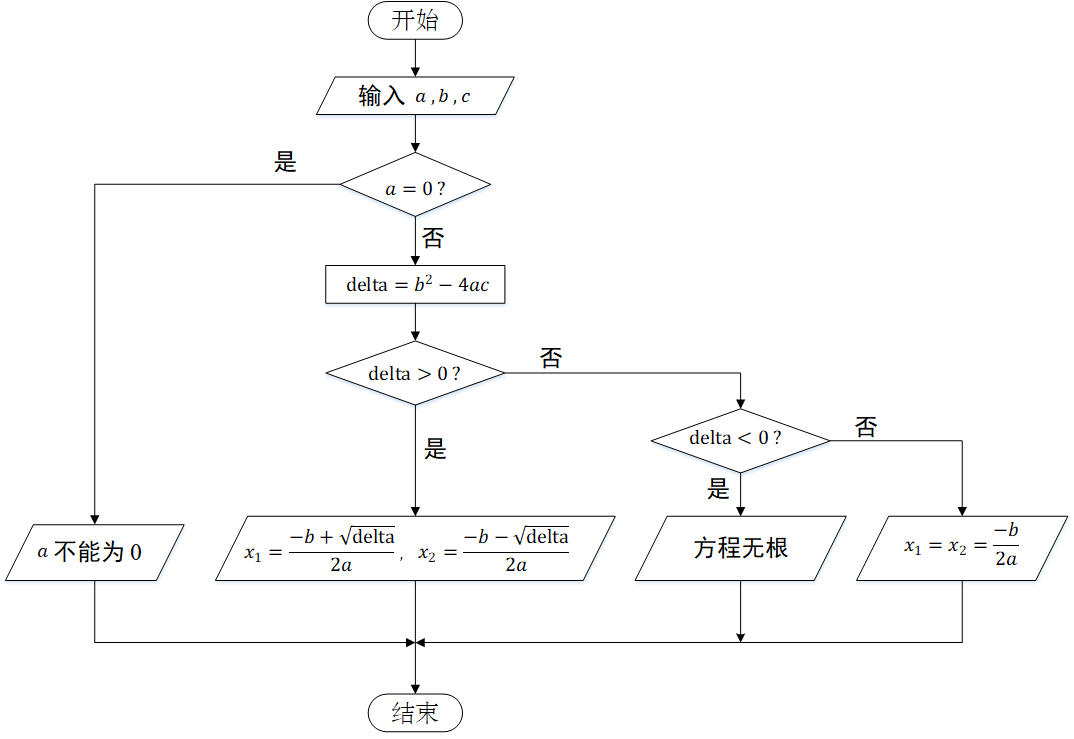
\includegraphics[scale=0.3]{example3_3.png}
			\end{figure}
\end{frame}

\begin{frame}[fragile]
	\frametitle{3.2 分支结构\small{—\texttt{if}语句}}
	% \framesubtitle{——\texttt{if}语句}
	\begin{exampleblock}{代码清单3.3,例3.3:}
\vspace{-3mm}
		\begin{columns}
			\begin{column}{0.06\linewidth}
			\end{column}
			\begin{column}{0.94\linewidth}
				\begin{lstlisting}[numbers=left,numberstyle=\small,basicstyle=\small\ttfamily]
#include<iostream>
#include<cmath>                         //用于求平方根函数sqrt,第12行代码
using namespace std;
int main() {
    double a,b,c;                       //创建3个double类型对象存放三个系数值
    cout << "请输入a,b,c:";
    cin >> a >> b >> c;
    if (a != 0) {
        double delta = b*b - 4 * a*c;
        if (delta > 0) {
            double x1, x2;              //需要时创建对象
            delta = sqrt(delta);        //求delta的平方根
            x1 = (-b + delta) / (2 * a);
            x2 = (-b - delta) / (2 * a);
            cout << "方程有两个实根:" << x1 << ", " << x2 << endl;
        }
                \end{lstlisting}\ttfamily
			\end{column}
		\end{columns}
	\end{exampleblock}
\end{frame}

\begin{frame}[fragile]
	\frametitle{3.2 分支结构\small{—\texttt{if}语句}}
	% \framesubtitle{——\texttt{if}语句}
	\begin{exampleblock}{代码清单3.3,例3.3:}
		\begin{columns}
			\begin{column}{0.06\linewidth}
			\end{column}
			\begin{column}{0.94\linewidth}
				\begin{lstlisting}[numbers=left,numberstyle=\small,firstnumber=17,basicstyle=\small\ttfamily]
        else if (delta < 0) {
            cout << "方程无实根" << endl;
        }
        else {
            cout << "方程有两个相同的实根:" << -b / (2 * a) << endl;
        }
    }
    else {                          //二次项系数不能为0
        cout << "a不能为0" << endl;
    }
    return 0;
}
    \end{lstlisting}\ttfamily
			\end{column}
		\end{columns}
		\ttfamily 示例:输入\texttt{a~=~1,~b~=~-4,~c~=~4}~~~输出:方程有两个相同的实根:2
	\end{exampleblock}
\end{frame}


\begin{frame}[fragile]
	\frametitle{3.2 分支结构\small{—\texttt{switch}语句}}
	% \framesubtitle{——\texttt{switch}语句}
	\begin{columns}
\vspace{-3mm}
		\begin{column}{0.3\linewidth}
		\end{column}
		\begin{column}{0.4\linewidth}
			\begin{block}{\texttt{switch}分支结构格式:}
				\begin{lstlisting}[basicstyle=\small\ttfamily]
  /*...*/
  int score;
  cin >> score;
  switch (score/10){
  case 9:
      cout << "A" << endl;
      break;
  case 8:
      cout << "B" << endl;
      break;
  ...
  default;
      cout << "F" << endl;
  }
  /*...*/
        \end{lstlisting}
			\end{block}
		\end{column}
		\begin{column}{0.3\linewidth}
		\end{column}
	\end{columns}
\end{frame}

\begin{frame}[fragile]
	\frametitle{3.2 分支结构\small{—\texttt{switch}语句}}
	% \framesubtitle{——\texttt{switch}语句}

	\begin{block}{\texttt{switch}语句语法规则:}
		\begin{itemize}
			\item 每个开关入口可以\alert{对应多个标签值},执行相同的操作,\alert{标签值后紧接冒号}\\
			      \begin{lstlisting}[basicstyle=\small\ttfamily]
        /*...*/
        switch(score/10){
        case 9: case 10:
            cout << "A" << endl;
            break;
        /*...*/
        \end{lstlisting}
			\item \texttt{case}标签的值\alert{必须为整型常量},且每个\alert{标签值必须不同},否则会引发语法错误:\\
			      \begin{lstlisting}[basicstyle=\small\ttfamily]
        case 9.0:case 10:           //报错:表达式必须为整型常量表达式
            cout << "A" << endl;
            break;
        case 10:                    //报错:标签值已经出现
            cout << "B" << endl;
            break;
            \end{lstlisting}
		\end{itemize}
	\end{block}
\end{frame}

\begin{frame}[fragile]
	\frametitle{3.2 分支结构\small{—\texttt{switch}语句}}
	% \framesubtitle{——\texttt{switch}语句}

	\begin{block}{\texttt{switch}语句语法规则:}
		\begin{itemize}
			\item \texttt{break}~语句需根据需要谨慎选择。如果因疏忽,忘记~\texttt{break}~语句,可能带来灾难性的逻辑错误:\\
			      \begin{lstlisting}[basicstyle=\small\ttfamily]
        /*...*/
        case 8:
            cout << "B" << endl;
        case 7:
            cout << "C" << endl;
            break;
        /*...*/
        \end{lstlisting}
			      当~\texttt{score}~在\texttt{B}分数段内时,比如85分,会得到如下错误的输出:\\
			      \texttt{B\\
				      C}
		\end{itemize}
	\end{block}
\end{frame}

\begin{frame}[fragile]
	\frametitle{3.2 分支结构\small{—\texttt{switch}语句}}
	% \framesubtitle{——\texttt{switch}语句}

	\begin{block}{\texttt{switch}语句语法规则:}
		\begin{itemize}
			\item 开关语句里面\alert{初始化}对象时需要使用花括号,否则出现语法错误。
			      例如:\\
			      \begin{lstlisting}[basicstyle=\small\ttfamily]
        case 8:
            char c = 'B';       //初始化
            break;
        case 7:
            c = 'C';  //修改在前面标签处定义的对象
            break;
            \end{lstlisting}
            进入开关case 7时,前面开关case 8 被跳过,造成对象c未定义,出现错误
		\end{itemize}
	\end{block}
\end{frame}

\begin{frame}[fragile]
	\frametitle{3.2 分支结构\small{—\texttt{switch}语句}}
	% \framesubtitle{——\texttt{switch}语句}

	\begin{block}{\texttt{switch}语句语法规则:}
		\begin{itemize}
			\item 开关语句里面定义对象时需要使用花括号。
			      例如:\\
			      \begin{lstlisting}[basicstyle=\small\ttfamily]
        case 8:{
            char c = 'B';   //对象c只在case 8的作用域内可见
            break;
        }
        case 7:
            c = 'C';        //修改在前面标签处定义的对象,报错
            break;
            \end{lstlisting}
             编译错误,case 7处对象c未定义
		\end{itemize}
	\end{block}
\end{frame}

\begin{frame}[fragile]
	\frametitle{3.2 分支结构\small{—\texttt{switch}语句}}
	% \framesubtitle{——\texttt{switch}语句}
	\begin{exampleblock}{代码清单3.4,使用\texttt{switch}语句解决例3.2}
\vspace{-3mm}
		\begin{columns}[t]
			\begin{column}{0.04\linewidth}
			\end{column}
			\begin{column}{0.4\textwidth}
				\begin{lstlisting}[numbers=left,numberstyle=\small,basicstyle=\small\ttfamily]
#include<iostream>
using namespace std;
int main() {
    int score;
    cout << "请输入一个分数:";
    cin >> score;
    //整型值表达式
    switch (score/10){
    case 9:case 10:
        cout << "A" << endl;
        break;
    //常量标签值后面紧跟冒号
    case 8:
        cout << "B" << endl;
        \end{lstlisting}\ttfamily
			\end{column}
			\begin{column}{0.1\linewidth}
			\end{column}
			\begin{column}{0.4\textwidth}
				\begin{lstlisting}[numbers=left,numberstyle=\small,firstnumber=15,basicstyle=\small\ttfamily]
        break;
    case 7:
        cout << "C" << endl;
        break;
    case 6:
        cout << "D" << endl;
        break;
    default:
        cout << "F" << endl;
        break;
    }
    return 0;
}
        \end{lstlisting}\ttfamily
			\end{column}
		\end{columns}
		\ttfamily 示例:输入:76~~~输出:\texttt{C}
	\end{exampleblock}
\end{frame}

\begin{frame}[fragile]
	\frametitle{3.3 循环结构}
	% \framesubtitle{——if 语句}
	\begin{abstractblock}{三种循环结构:}
		\begin{itemize}
			\item \textcolor[rgb]{0,0,1}{\texttt{while}}语句
			\item \textcolor[rgb]{0,0,1}{\texttt{do while}}语句
			\item \textcolor[rgb]{0,0,1}{\texttt{for}}语句
		\end{itemize}
	\end{abstractblock}
\end{frame}

\begin{frame}[fragile]
	\frametitle{3.3 循环结构\small{—\texttt{while}语句}}
	% \framesubtitle{——\texttt{while}语句}
	\begin{columns}
		\begin{column}{0.48\textwidth}
			\begin{block}{\texttt{while}语句语法格式}
				\begin{lstlisting}[basicstyle=\small\ttfamily]
while (expr) { //条件表达式
    statement; //循环体语句
}
                \end{lstlisting}\ttfamily
			\end{block}
		\end{column}
		\hfill
		\begin{column}{0.4\textwidth}
			\begin{figure}[ht]
				\centering
				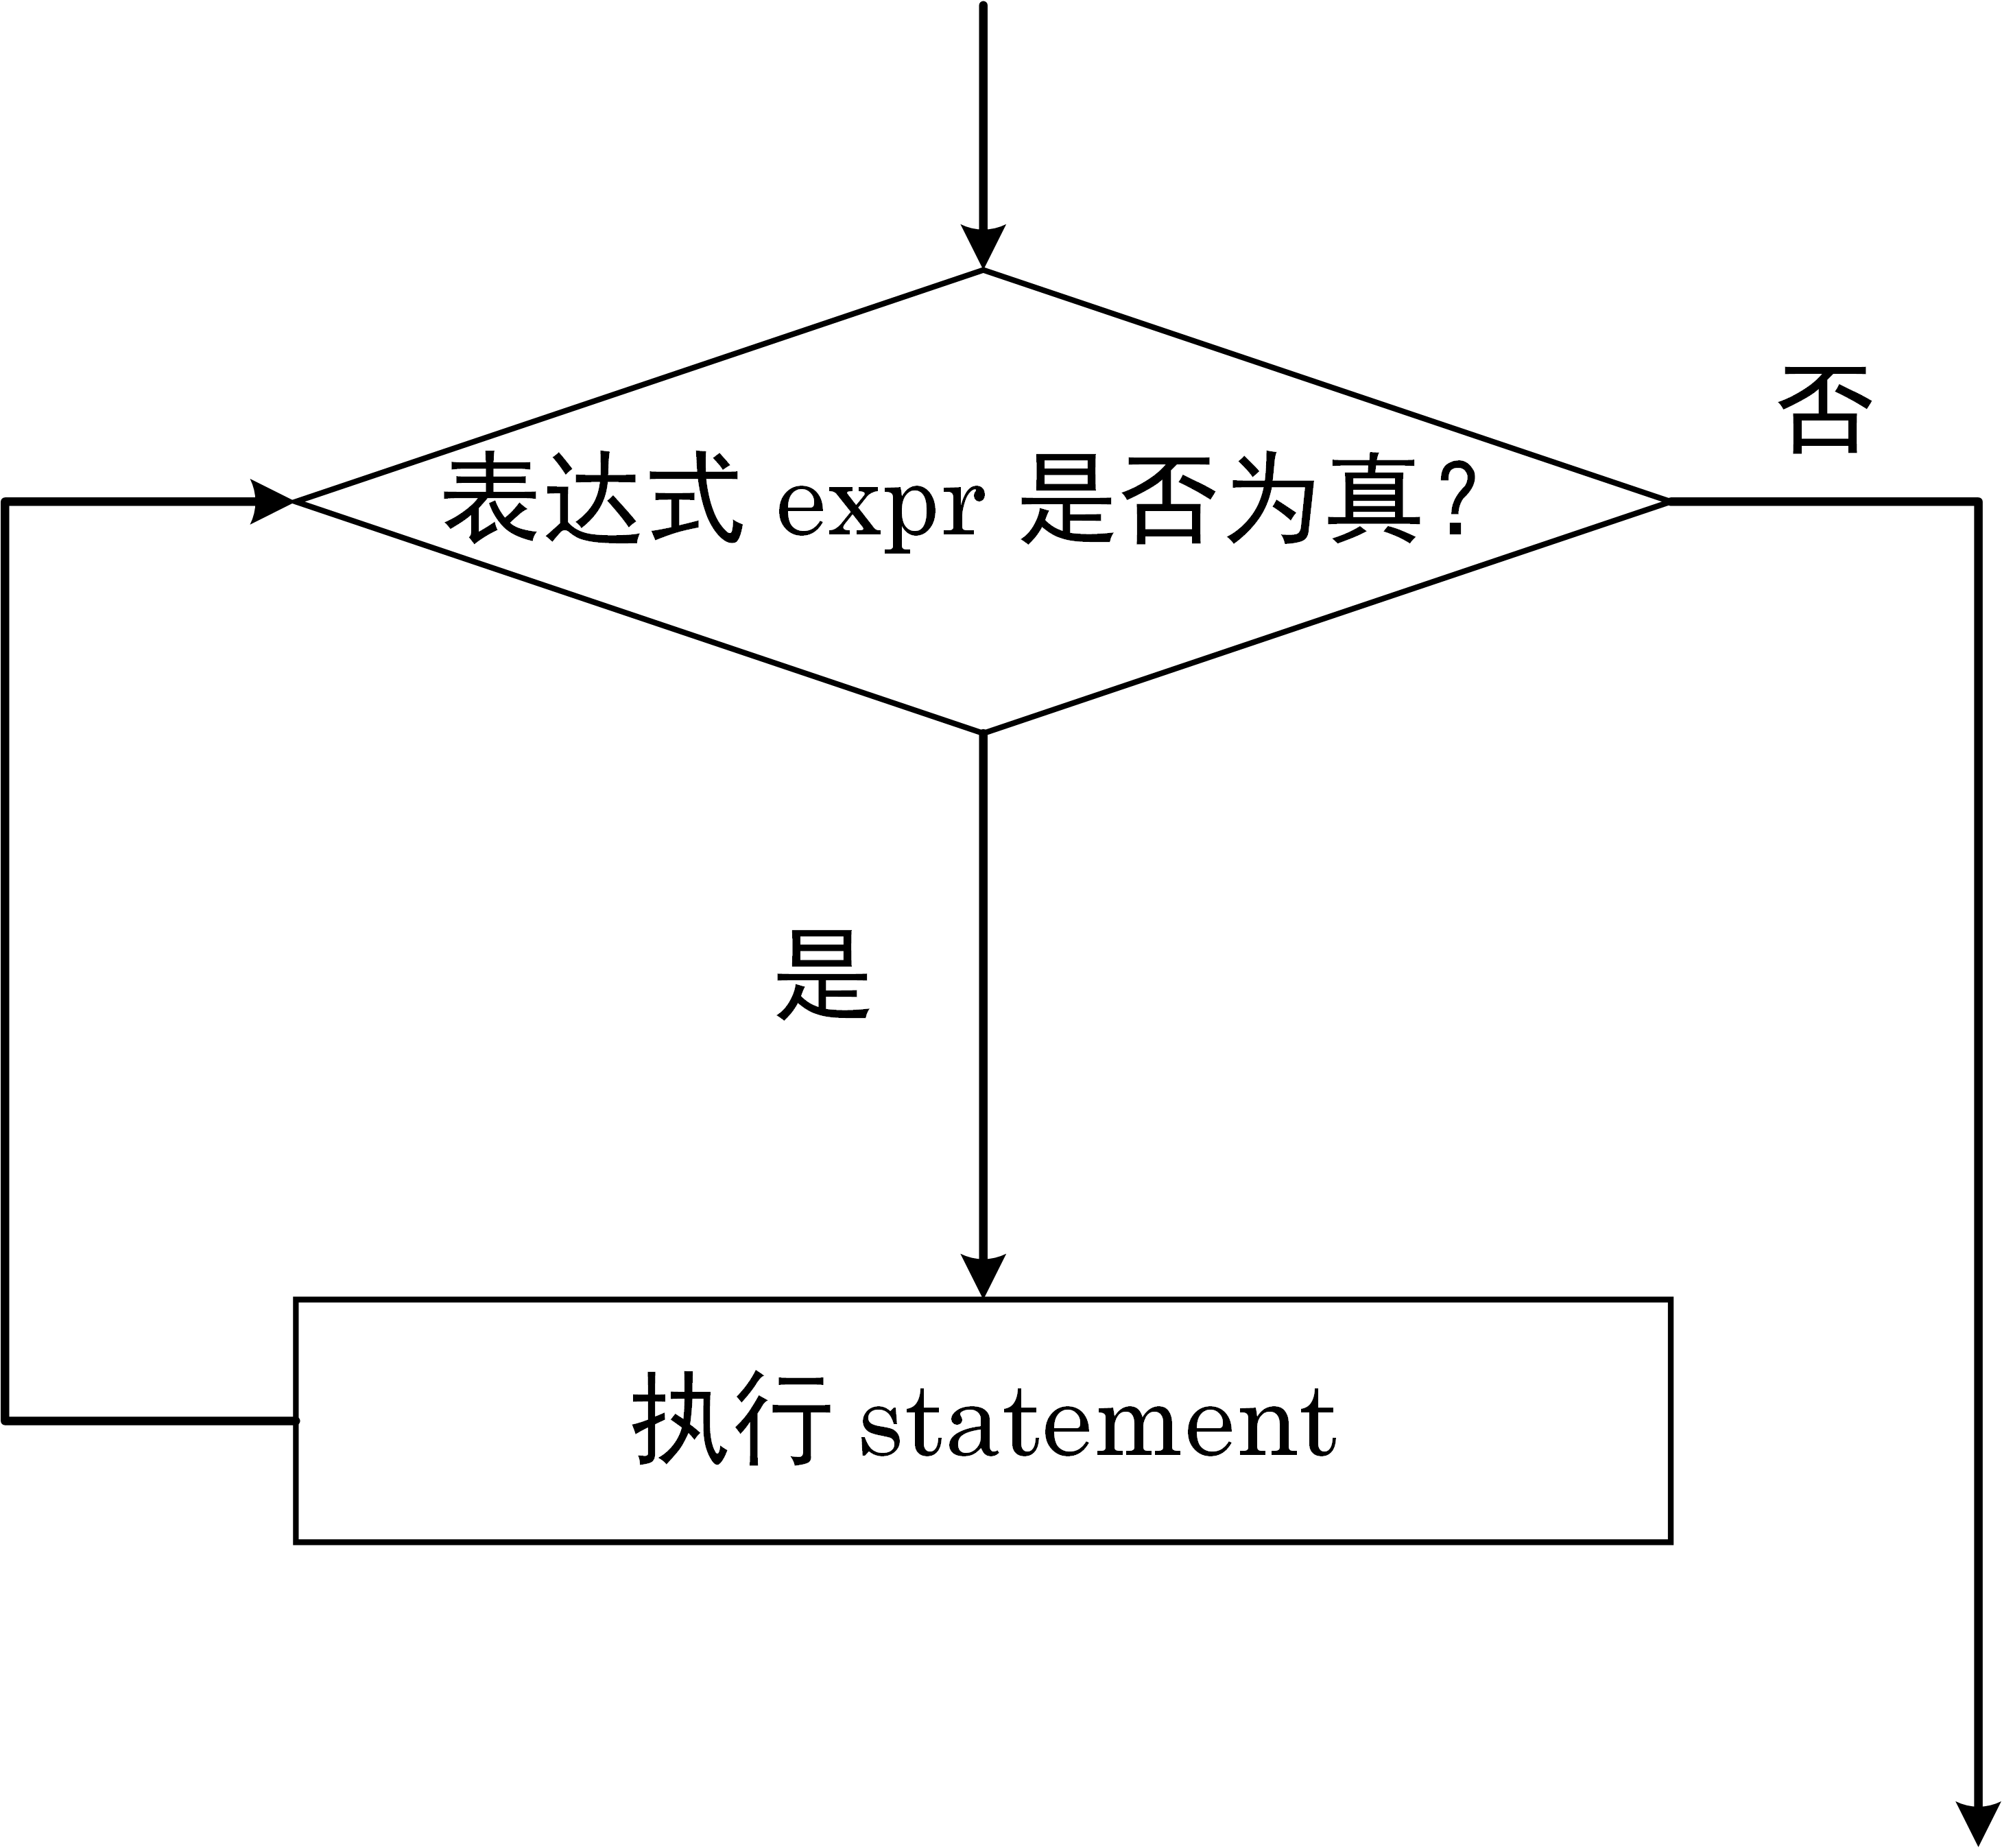
\includegraphics[scale=0.4]{while_statement.png}
				% \caption{\texttt{while}语句执行流程}
				% \label{fig:label}
			\end{figure}
		\end{column}
	\end{columns}
\end{frame}
\begin{frame}[fragile]
	\frametitle{3.3 循环结构\small{—\texttt{while}语句}}
	% \framesubtitle{——\texttt{while}语句}
	\begin{exampleblock}{练习:}
		下面程序段的运行结果是多少?
		\begin{lstlisting}[basicstyle=\small\ttfamily]
        int x = 0, y = 0;
        while (x < 15) {
            ++y;
            x += 1;
        }
        cout << y << endl;
    \end{lstlisting}\ttfamily
		\ttfamily \onslide<2->{答案:15}
	\end{exampleblock}
\end{frame}
\begin{frame}[fragile]
	\frametitle{3.3 循环结构\small{—\texttt{while}语句}}
	% \framesubtitle{——\texttt{while}语句}
	\begin{exampleblock}{例3.4:}
		\ttfamily
		根据以下公式利用迭代法求~$\pi$~的近似值,最后一项小于或等于~1.0E-10~时停止。\\
		\begin{center}\[\frac{\pi}{2}= 1+\frac{1}{3}+\frac{1}{3}\times\frac{2}{5}+\frac{1}{3}\times\frac{2}{5}\times\frac{3}{7}+\ldots+ x_{i}, ~~x_{i}=x_{i-1}\times\frac{i-1}{2i-1}\]
		\end{center}
	\end{exampleblock}
\end{frame}

\begin{frame}[fragile]
	\frametitle{3.3 循环结构\small{—\texttt{while}语句}}
	% \framesubtitle{——\texttt{while}语句}
	\begin{exampleblock}{代码清单3.5,例3.4:}
\vspace{-3mm}
		\begin{columns}
			\begin{column}{0.06\linewidth}
			\end{column}
			\begin{column}{0.94\textwidth}
				\begin{lstlisting}[numbers=left,numberstyle=\small,basicstyle=\small\ttfamily]
#include<iostream>
#include <iomanip>          //库函数setprecision
using namespace std;
int main() {
    double sum=0,x=1;       //sum存放数列前i项的和, x存放当前项的值,注意初始值
    int i = 1;              //求解第i项
    while (x > 1.0E-10) {
        sum += x;
        ++i;                //在当前项基础上计算下一项
        x *= (i - 1.) / (2 * i - 1);    //注意1后面的小数点
    }
    //fixed和setprecision用于控制输出精度,输出结果pi=3.1415926533
    cout<<"pi="<<fixed<<setprecision(10)<<2*sum<<endl;
    return 0;
}
\end{lstlisting}\ttfamily
			\end{column}
		\end{columns}
	\end{exampleblock}
\end{frame}

\begin{frame}[fragile]
	\frametitle{3.3 循环结构\small{—\texttt{do while}语句}}
	% \framesubtitle{——\texttt{do while}语句}
	\begin{columns}
		\begin{column}{0.55\textwidth}
			\begin{block}{\texttt{do while}语句语法格式}
				\begin{lstlisting}[basicstyle=\small\ttfamily]
do{
    statement; //循环体语句
}while (expr); //条件表达式,注意以分号结束
                \end{lstlisting}\ttfamily
			\end{block}
		\end{column}
		\begin{column}{0.4\textwidth}
			\begin{figure}[ht]
				\centering
				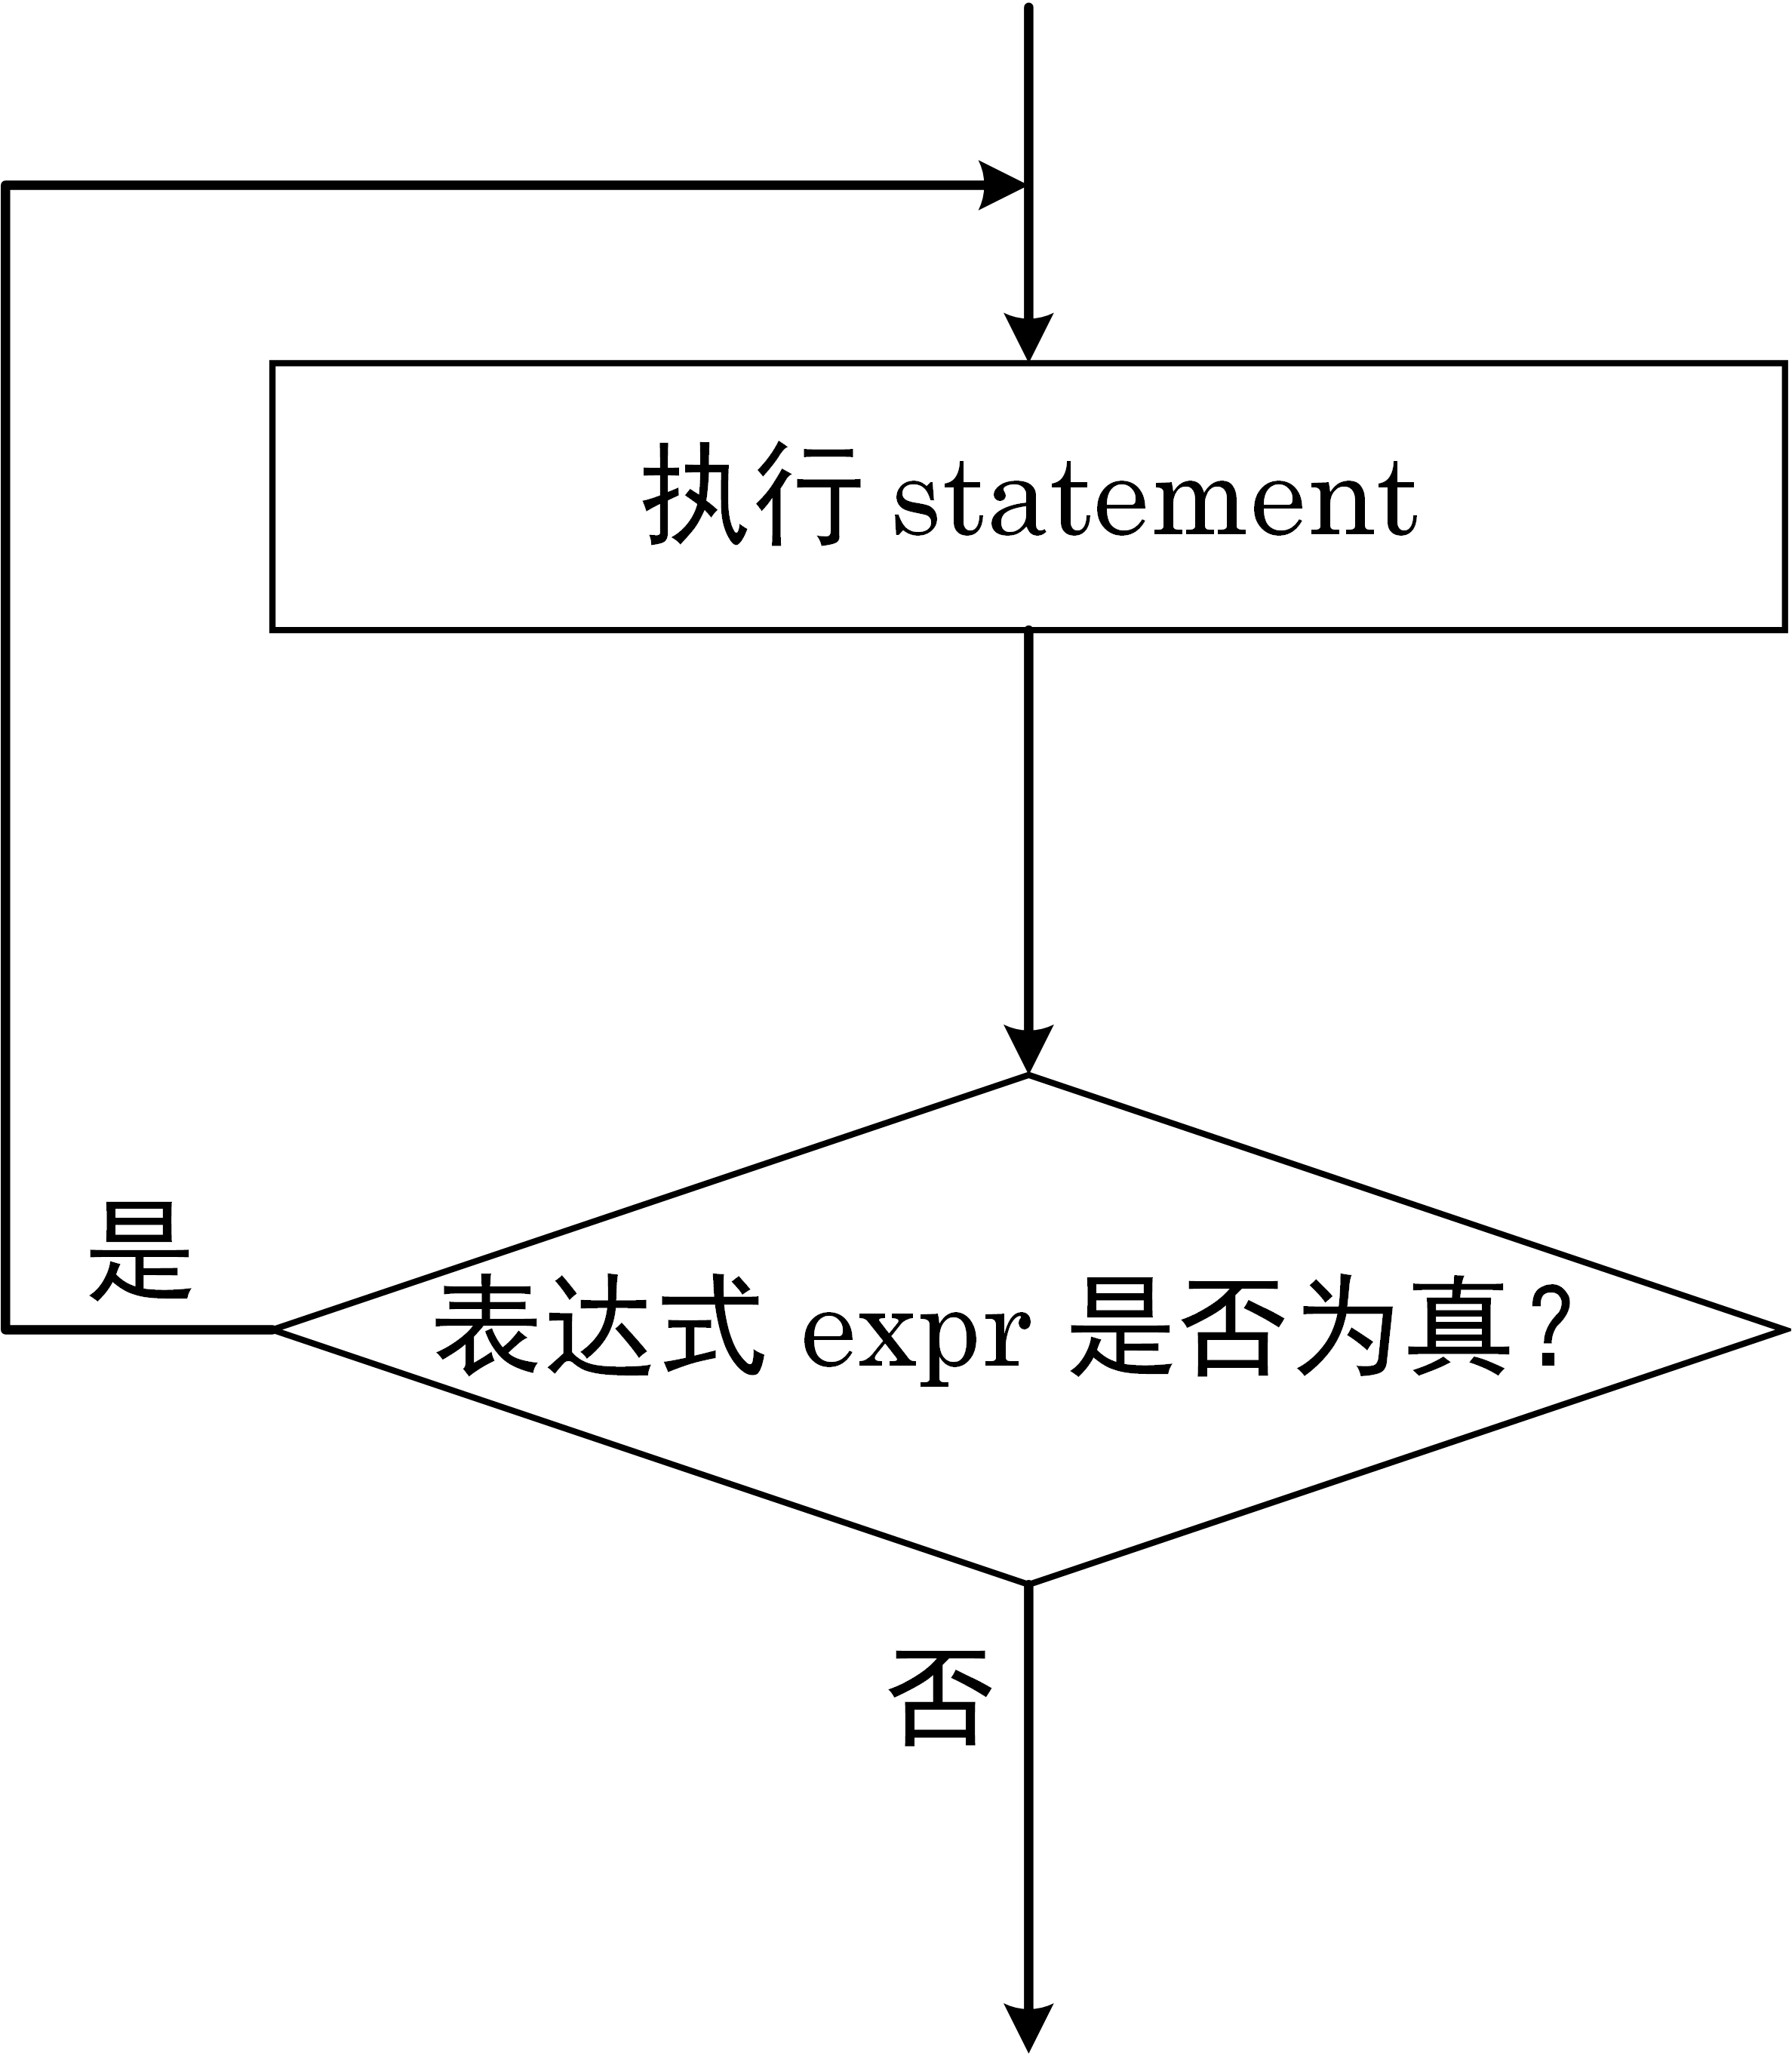
\includegraphics[scale=0.5]{dowhile_statement.png}
				% \caption{\texttt{do while}语句执行流程}
				% \label{fig:label}
			\end{figure}
		\end{column}
	\end{columns}
\end{frame}

\begin{frame}[fragile]
	\frametitle{3.3 循环结构\small{—\texttt{do while}语句}}
	% \framesubtitle{——\texttt{do while}语句}
	\begin{columns}
		\begin{column}{0.5\textwidth}
			\begin{exampleblock}{例3.5:}
				\ttfamily 输入一段文本,统计数字字符个数。\\
				\quad\\
				\alert{提示}:程序主要流程如右图所示
			\end{exampleblock}
		\end{column}
		\begin{column}{0.4\textwidth}
			\begin{figure}[ht]
				\centering
				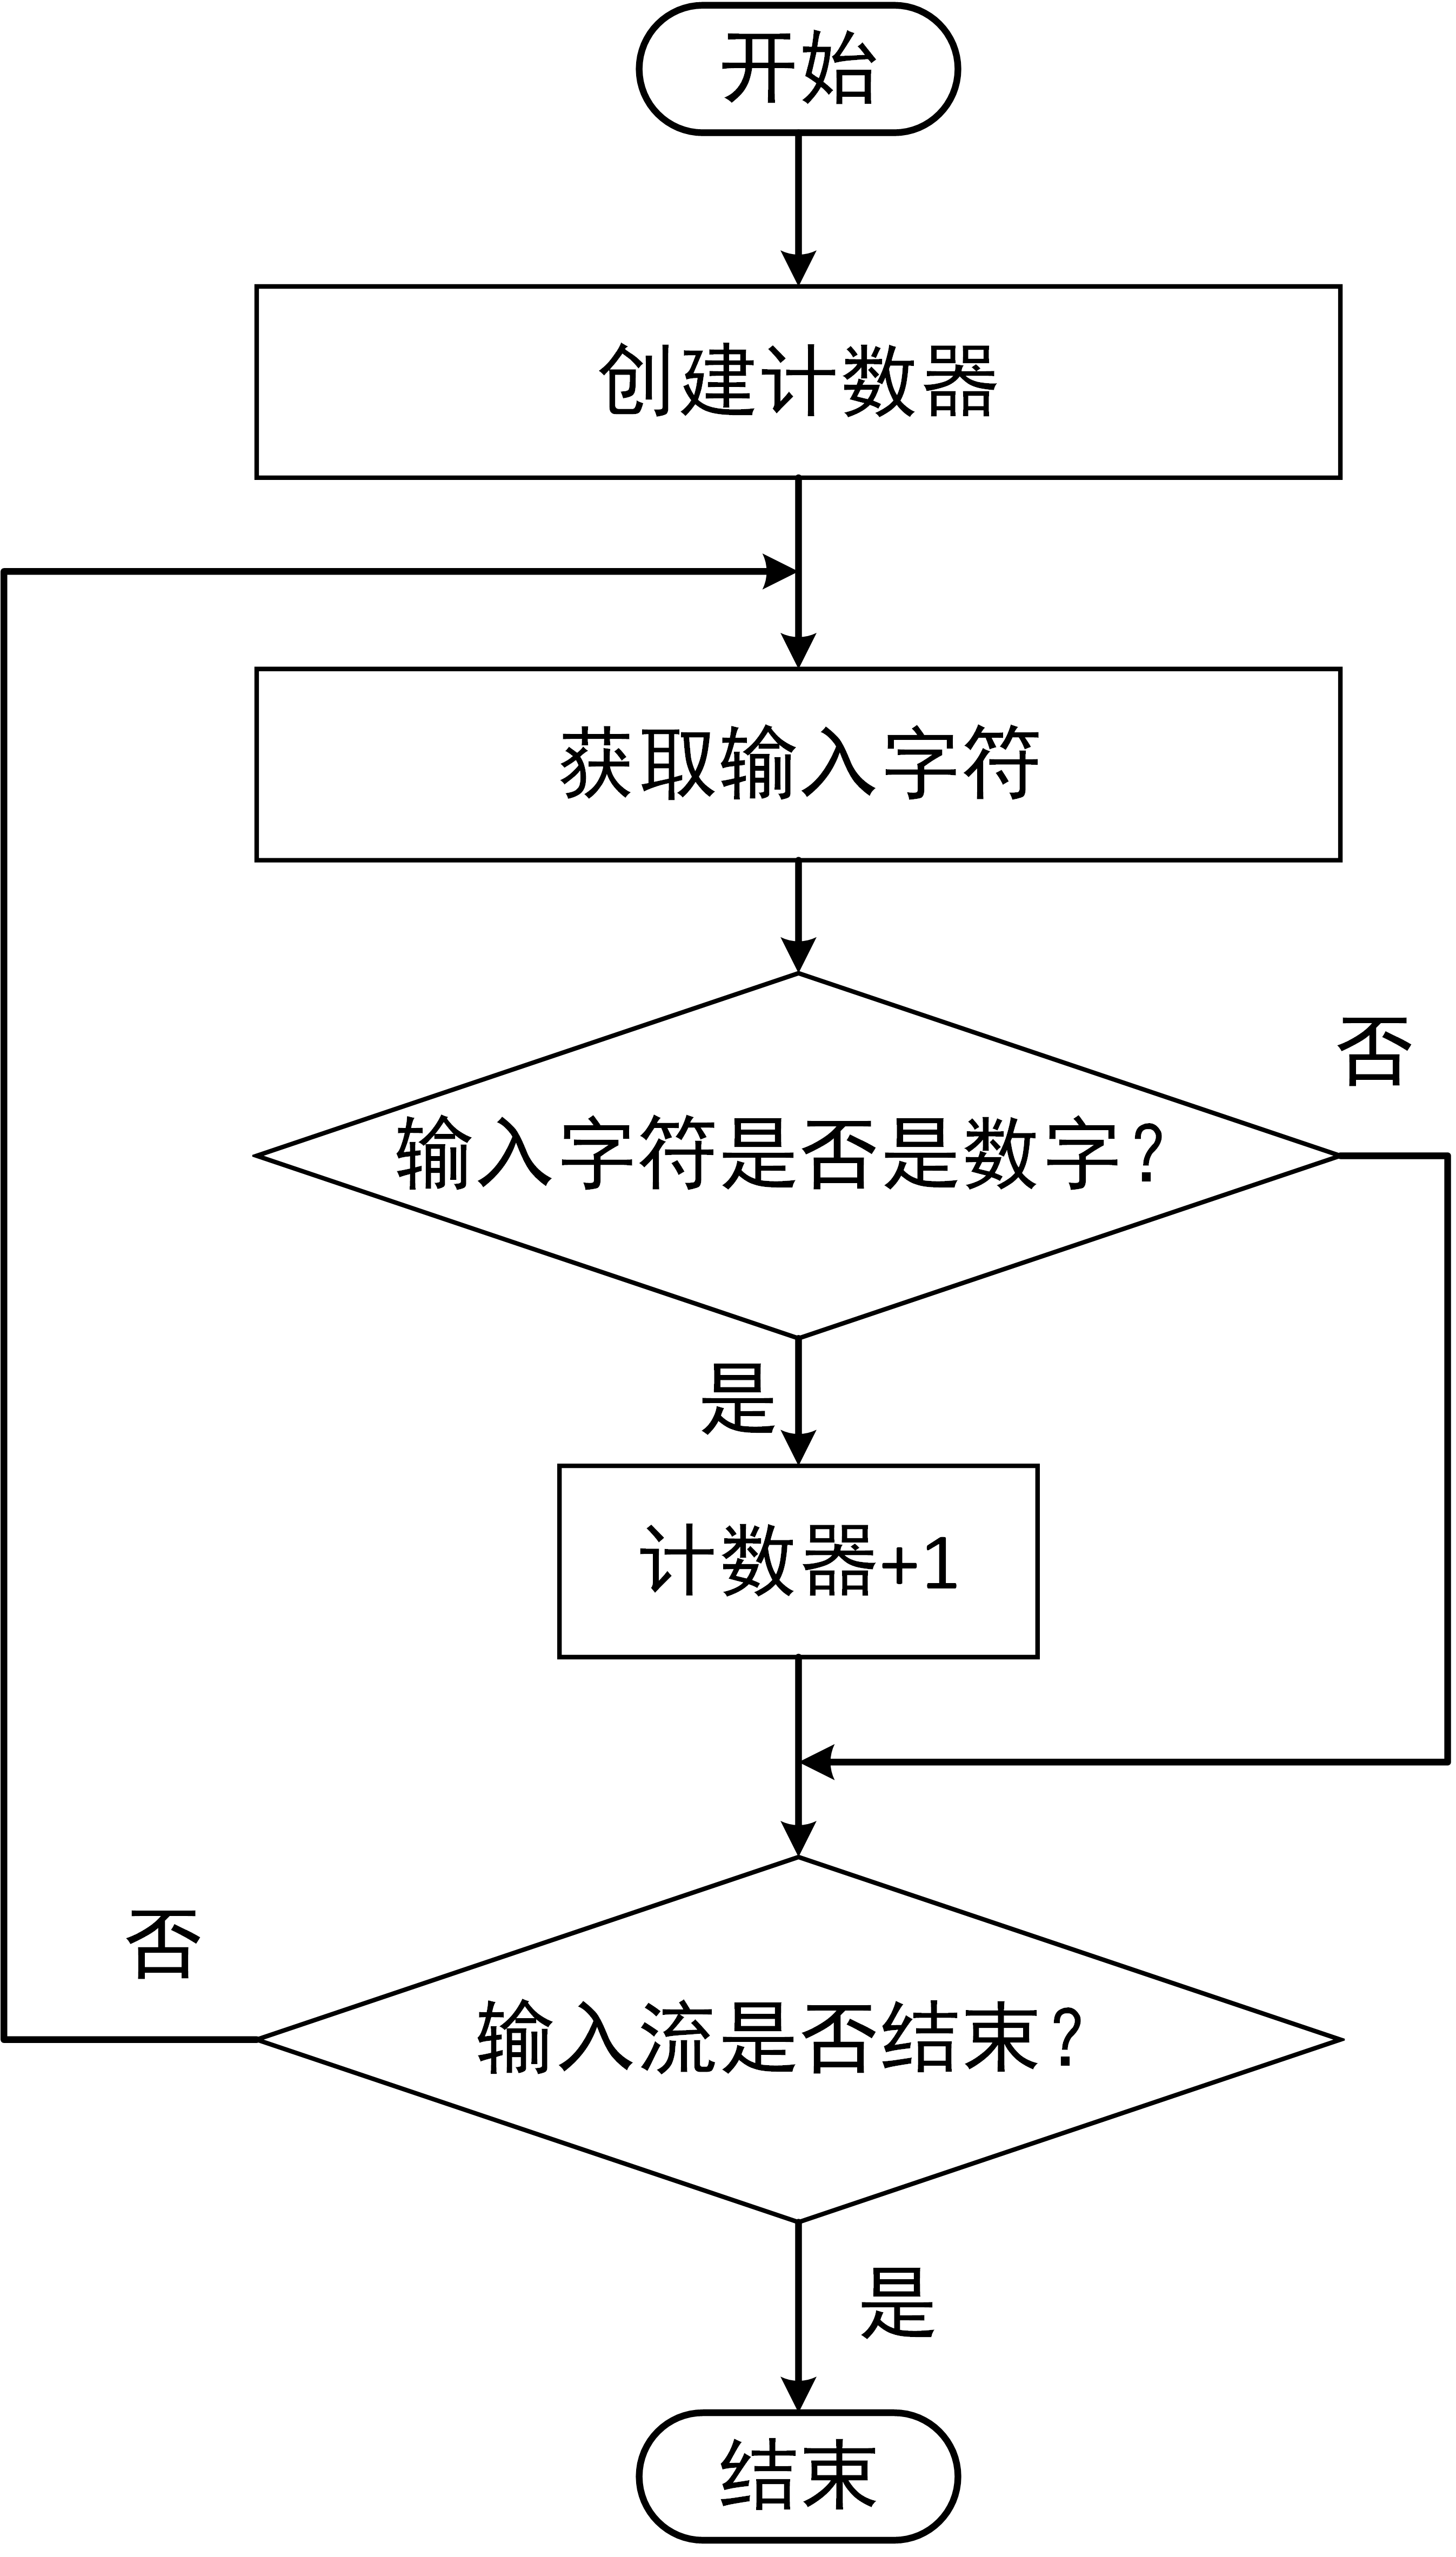
\includegraphics[scale=0.38]{example3_5.png}
				% \caption{\texttt{do while}语句执行流程}
				% \label{fig:label}
			\end{figure}
		\end{column}
	\end{columns}
\end{frame}

\begin{frame}[fragile]
	\frametitle{3.3 循环结构\small{—\texttt{do while}语句}}
	% \framesubtitle{——\texttt{do while}语句}
	\begin{exampleblock}{代码清单3.6,例3.5:}
		\begin{columns}
			\begin{column}{0.06\linewidth}
			\end{column}
			\begin{column}{0.94\textwidth}
				\begin{lstlisting}[numbers=left,numberstyle=\small,basicstyle=\small\ttfamily]
#include<iostream>
using namespace std;
int main() {
    int cnt = 0;
    char x;
    do {
        x = cin.get();  //获取终端输入的任意一个字符
        if (x >= '0'&&x <= '9') ++cnt;
    } while (x != EOF); //EOF为输入流结束标志,组合键Ctrl+Z
    cout << "数字字符个数为: " << cnt << endl;
    return 0;
}
\end{lstlisting}
			\end{column}
		\end{columns}
		\ttfamily 输入:ab12345~~~输出:数字字符个数为:5
	\end{exampleblock}
\end{frame}


\begin{frame}[fragile]
	\frametitle{3.3 循环结构\small{—\texttt{do while}语句}}
	% \framesubtitle{——\texttt{do while}语句}
	\begin{exampleblock}{练习:}
\begin{columns}
\column{0.5\textwidth}
		\ttfamily 1.下面程序段中的循环执行几次?
		\begin{lstlisting}[basicstyle=\small\ttfamily]
    int x = -1;
    do{
        x = x * x;
    }while(!x);
                \end{lstlisting}
\indent		A.死循环~~~~~B.执行3次~~\\C.执行1次~~D.有语法错误
\column{0.5\textwidth}
		 2.下面程序段的输出结果是?
		\begin{lstlisting}[basicstyle=\small\ttfamily]
    int y = 10;
    do{
        y--;
    }while(--y);
    cout << y-- << endl;
    \end{lstlisting}

\indent		A.~-1~~~~B.~1~~~~C.~8~~~~D.~0
\end{columns}
\bigskip
		\onslide<2->{答案:1.C~~2.D}
	\end{exampleblock}
\end{frame}


\begin{frame}[fragile]
	\frametitle{3.3 循环结构\small{—\texttt{for}语句}}
	% \framesubtitle{——\texttt{for}语句}
	\begin{columns}
		\begin{column}{0.45\textwidth}
			\begin{block}{\texttt{for}语句语法格式}
				\begin{lstlisting}[basicstyle=\small\ttfamily]
for(expr1; expr2; expr3){
    statement;
}
                \end{lstlisting}
				\ttfamily 例如,1到100累加求和:
				\begin{lstlisting}[basicstyle=\small\ttfamily]
int sum = 0;
for(int i = 1; i <= 100; ++i){
    sum += i;
}
        \end{lstlisting}
			\end{block}
		\end{column}
		\begin{column}{0.45\textwidth}
			\begin{figure}[ht]
				\centering
				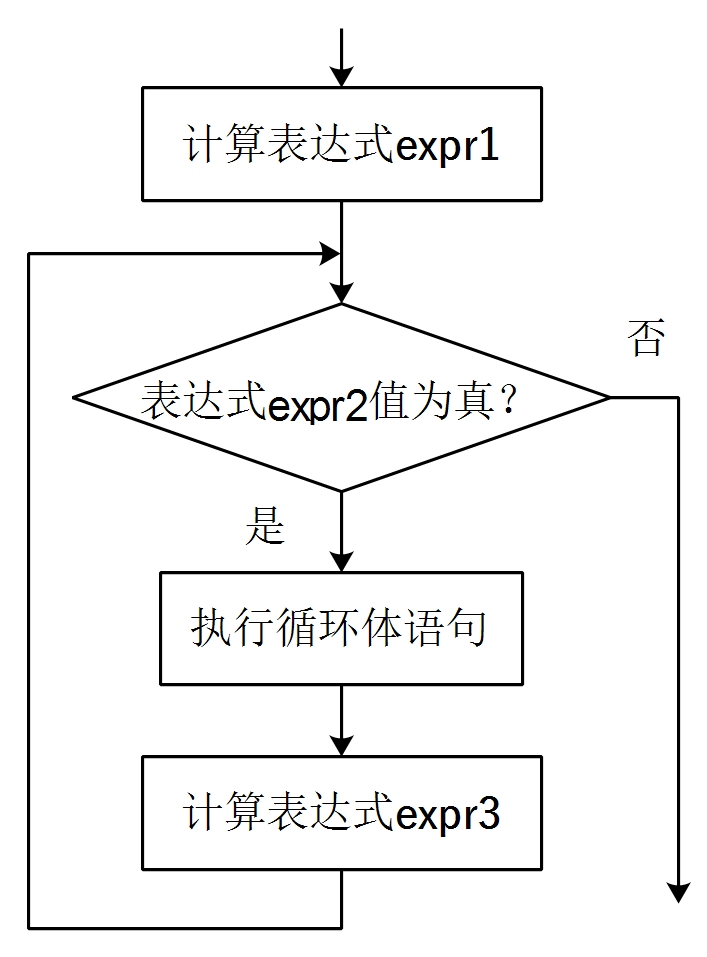
\includegraphics[scale=0.8]{Fig3-1.jpg}
				% \caption{\texttt{for}语句执行流程}
				% \label{fig:label}
			\end{figure}
		\end{column}
	\end{columns}
\end{frame}

\begin{frame}[fragile]
	\frametitle{3.3 循环结构\small{—\texttt{for}语句}}
	% \framesubtitle{——\texttt{for}语句}
	\begin{block}{\texttt{for}非常灵活,可以有多种形式}
		\begin{itemize}
			\item 可以省略任意一个表达式,但\alert{分号不能省略}:
		\end{itemize}
	\end{block}
	\begin{columns}
		\begin{column}[t]{0.32\linewidth}
			\begin{thinkblock}{}
				\texttt{int i(1),sum(0);}\\
				\texttt{for(; i<=100; ++i)\{}\\
				\texttt{\text{~~~} sum += i;}\\
				\texttt{\}}  \\
				\alert{//省略表达式\texttt{expr1}}
			\end{thinkblock}
		\end{column}
		\hfill
		\begin{column}[t]{0.32\linewidth}
			\begin{thinkblock}{}
				\texttt{int i(1),sum(0);}\\
				\texttt{for(; i<=100; )\{}\\
				\texttt{\text{~~~} sum += i++;}\\
				\texttt{\}~~//注意不是++i;}\\
				\alert{//省略\texttt{expr1}和\texttt{expr3}}
			\end{thinkblock}
		\end{column}
		\hfill
		\begin{column}[t]{0.32\linewidth}
			\begin{thinkblock}{}
				\texttt{int i(1),sum(0);}\\
				\texttt{for(; ; )\{}\\
				\texttt{\text{~~~} sum += i++;}\\
				\texttt{\text{~~~} if(i>100) break;}\\
				\texttt{\}}  \alert{//三个全部省略}\\
			\end{thinkblock}
		\end{column}
	\end{columns}
\end{frame}

\begin{frame}[fragile]
	\frametitle{3.3 循环结构\small{—\texttt{for}语句}}
	% \framesubtitle{——\texttt{for}语句}
	\begin{block}{\texttt{for}非常灵活,可以有多种形式}
		\begin{itemize}
			\item 表达式\texttt{expr1}可以\alert{定义多个对象},表达式\texttt{expr3}可以是任意表达式:
			      \begin{lstlisting}[basicstyle=\small\ttfamily]
for (int i = 1, j = 100; i < j; ++i, --j) {
    sum += i + j;
}
            \end{lstlisting}
		\end{itemize}
	\end{block}
	\begin{alertblock}{注意:}
		虽然上述表达式可以省略,但是需要在合适的位置添加相应功能的语句。
	\end{alertblock}
\end{frame}

\begin{frame}[fragile]
	\frametitle{3.3 循环结构\small{—\texttt{for}语句}}
	% \framesubtitle{——\texttt{for}语句}
	\begin{exampleblock}{练习:}
		\ttfamily 1.下面程序段中的循环执行几次?
		\begin{lstlisting}[basicstyle=\small\ttfamily]
    /*...*/
    int a,b;
    for(a = 0,b = 5;a <= b+1;a += 2,b--)
        cout << a << endl;
    /*...*/
                    \end{lstlisting}
		A.3~~B.2~~C.1~~D.0\\
		\onslide<2->{答案:A}
	\end{exampleblock}
\end{frame}

\begin{frame}[fragile]
	\frametitle{3.3 循环结构\small{—\texttt{for}语句}}
	% \framesubtitle{——\texttt{for}语句}
	\begin{exampleblock}{练习:}
		\ttfamily 2.下面程序段运行结束后,k的值是?
		\begin{lstlisting}[basicstyle=\small\ttfamily]
        int main() {
            int i, j, k;
            for (i = 0, j = 10; i <= j; i++, j--)
                k = i + j;
            cout << k << endl;
        }
        \end{lstlisting}
		A.0~~B.9~~C.8~~D.10\\
		\onslide<2->{答案:D}
	\end{exampleblock}
\end{frame}

\begin{frame}[fragile]
	\frametitle{3.3 循环结构}
	% \framesubtitle{——for 语句}
	\begin{exampleblock}{练习:}
		\ttfamily 3.下列语句中,哪一个不是无限循环?
		\begin{columns}
			\begin{column}[t]{0.4\linewidth}
				\begin{lstlisting}[basicstyle=\small\ttfamily]
A. i=100;
    while(1)
    { i=i%100; i++;
      if (i > 100) break;
    }
    \end{lstlisting}
				\begin{lstlisting}[basicstyle=\small\ttfamily]
C. short k=32765;
    do {
        k++; k++;
    }while(k>0);

        \end{lstlisting}
			\end{column}
			\hfill
			\begin{column}[t]{0.4\linewidth}
				\begin{lstlisting}[basicstyle=\small\ttfamily]
B. for(; ;)
    \end{lstlisting}
				~\\
				~\\~\\~\\
				\begin{lstlisting}[basicstyle=\small\ttfamily]
D. short i=32765;
    while((i++%2)||(i%2))
        i++;
    \end{lstlisting}
			\end{column}
		\end{columns}
		\onslide<2->{答案:C}
	\end{exampleblock}
\end{frame}

\begin{frame}[fragile]
	\frametitle{3.3 循环结构}
	% \framesubtitle{——for 语句}
	\begin{block}{循环语句的选择原则}
		\begin{itemize}
			\item 循环次数\alert{确定},选择\alert{\texttt{for}语句}
			\item 循环次数\alert{不确定},选择\alert{\texttt{while}}或\alert{\texttt{do while}语句}
			      \begin{itemize}
				      \item 循环体\alert{至少执行一次},选择\alert{\texttt{do while}语句}
				      \item 循环体\alert{一次也不执行},选择\alert{\texttt{while}语句}
			      \end{itemize}
		\end{itemize}
	\end{block}
\end{frame}

\begin{frame}[fragile]
	\frametitle{3.2 循环结构}
	% \framesubtitle{——do while 语句}
	\begin{exampleblock}{例3.6:}
		\ttfamily 猜数字游戏。程序随机选择一个0-100之间的一个数,玩家来猜测程序选择的数,如果猜对了,游戏结束,否则玩家继续猜测,直到猜中为止。对于玩家的每一次猜测,需要给出相应的提示信息:猜对了、猜大了或猜小了。\\
		\quad\\
		\alert{提示}:根据猜测次数,选择合适的循环语句
	\end{exampleblock}
\end{frame}

\begin{frame}[fragile]
	\frametitle{3.3 循环结构}
	% \framesubtitle{——do while 语句}
	\begin{exampleblock}{代码清单3.7,例3.6:}
		\begin{columns}
			\begin{column}{0.06\linewidth}
			\end{column}
			\begin{column}{0.94\textwidth}
\vspace{-5mm}
				\begin{lstlisting}[numbers=left,numberstyle=\small,basicstyle=\small\ttfamily]
int main(){
    srand(time(0));//系统当前时间作为随机数发生器的种子
    int target = rand() % 100;//获取一个[0-100)内的随机数
    int guess;
    cout << "`请猜0-100之内的数`" << endl;
    do {
        cin >> guess;
        if (guess < target) {
            cout << "猜小了" << endl;
        }else if(guess > target) {
            cout << "猜大了" << endl;
        }else {
            cout << "恭喜!猜对了!" << endl;
        }
    } while (guess != target); //猜中时游戏结束
}
\end{lstlisting}\ttfamily
			\end{column}
		\end{columns}
	\end{exampleblock}
\end{frame}

\begin{frame}[fragile]
	\frametitle{3.4 跳转语句}
	% \framesubtitle{——if 语句}
	\begin{abstractblock}{跳转语句用于中断当前的执行顺序,包括:}
		\begin{itemize}
			\item \textcolor[rgb]{1,0,0}{\texttt{break}}语句
			
			\item<2-> \textcolor[rgb]{1,0,0}{\texttt{continue}}语句
\item<3-> \textcolor[rgb]{0,0,0}{\texttt{return}}语句:
			      \begin{lstlisting}[basicstyle=\small\ttfamily]
    int main(){
        return 0; /*返回一个整型值*/
    }
\end{lstlisting}\ttfamily
			\item<4-> \texttt{goto}语句(不作介绍)
		\end{itemize}
	\end{abstractblock}
\end{frame}

\begin{frame}[fragile]
	\frametitle{3.4 跳转语句\small{—\texttt{break}语句}}
	% \framesubtitle{——\texttt{break}语句}
	\begin{block}{\texttt{break}语句}
		\alert{\texttt{break}~语句}只能用于\alert{~\texttt{switch}~语句}或\alert{循环语句}中,用来跳出离它最近的~\texttt{switch}~语句或终止循环的执行,它的作用域仅限离它最近的~\texttt{switch}~语句或循环语句。
	\end{block}
	\begin{exampleblock}{练习:}
		\ttfamily 1.下面程序段的运行结果是?
		\begin{columns}
			\begin{column}{0.65\linewidth}
				\begin{lstlisting}[basicstyle=\small\ttfamily]
    int a = 10, y = 0;
    do {
        a += 2;
        y += a;
        cout<<"a="<<a<<","<<"y="<<y<< endl;
        if (y > 50) break;
    } while (a = 14);
\end{lstlisting}
			\end{column}
			\begin{column}{0.3\linewidth}
				\onslide<2->{答案:\\a=12,y=12\\a=16,y=28\\a=16,y=44\\a=16,y=60}
			\end{column}
		\end{columns}
	\end{exampleblock}
\end{frame}

\begin{frame}[fragile]
	\frametitle{3.4 跳转语句\small{—\texttt{break}语句}}
	% \framesubtitle{——\texttt{break}语句}
	\begin{exampleblock}{示例:}
		\ttfamily 将例3.6改造成由~\texttt{while}~内嵌一个~\texttt{switch}~结构来说明~\texttt{break}~语句的用法\\
		~\\
		\alert{提示}:\texttt{switch}结构需要整型值表达式,可根据玩家猜测的数字与电脑给出的数字的大小关系进行转换
	\end{exampleblock}
\end{frame}


\begin{frame}[fragile]
	\frametitle{3.4 跳转语句\small{—\texttt{break}语句}}
	% \framesubtitle{——\texttt{break}语句}
	\begin{exampleblock}{代码清单3.8,例3.6:}
		\begin{columns}
\vspace{-3mm}
			\begin{column}{0.06\linewidth}
			\end{column}
			\begin{column}{0.94\textwidth}
\vspace{-3mm}
				\begin{lstlisting}[numbers=left,numberstyle=\small,basicstyle=\small\ttfamily]
#include <cstdlib>
#include <ctime>
int main(){
    srand(time(0));             //系统当前时间作为随机数发生器的种子
    int target = rand() % 100;  //获取一个0-100内的随机数
    int guess;
    cout << "`请猜0-100之内的数`" << endl;
    while(1) {
        cin >> guess;
        int val = (guess > target) - (guess < target);
                                //将guess和target的大小关系转化为三个数
        switch (val){
        case -1:
            cout << "猜小了" << endl;
            break;              //跳出switch
\end{lstlisting}\ttfamily
			\end{column}
		\end{columns}
	\end{exampleblock}
\end{frame}

\begin{frame}[fragile]
	\frametitle{3.4 跳转语句\small{—\texttt{break}语句}}
	% \framesubtitle{——\texttt{break}语句}
	\begin{exampleblock}{代码清单3.8,例3.6:}
		\begin{columns}
			\begin{column}{0.06\linewidth}
			\end{column}
			\begin{column}{0.94\textwidth}
				\begin{lstlisting}[numbers=left,numberstyle=\small,firstnumber=16,basicstyle=\small\ttfamily]
            case 1:
            cout << "猜大了" << endl;
            break;              //跳出switch
        default:
            cout << "恭喜! 猜对了!" << endl;
            break;              //跳出switch
        }                       //switch结束
        if (val == 0) {
            break;              //跳出while,游戏结束
        }
    }                           //while结束
    return 0;
}
\end{lstlisting}\ttfamily
			\end{column}
		\end{columns}
	\end{exampleblock}
\end{frame}

\begin{frame}[fragile]
	\frametitle{3.4 跳转语句\small{—\texttt{continue}语句}}
	% \framesubtitle{——\texttt{continue}语句}
	\begin{block}{\texttt{continue}语句}
		\alert{\texttt{continue}语句}只在\alert{循环结构}中有作用,用来终止当前操作,进入下一次循环。\texttt{continue}~ 语句的作用域仅作用于离它最近的循环
	\end{block}
	\begin{exampleblock}{例如:}\vspace{-3mm}
		\begin{lstlisting}[basicstyle=\small\ttfamily]
    //当i为奇数,输出*#,为偶数时无输出
    for (int i = 0; i < 5; ++i) {
        if (i % 2) {
            cout << "*"; //打印符号*,然后再打印符号#
        }
        else {
            continue; //结束当前迭代,跳转到for语句,执行++i
        }
        cout << "#";
    }
\end{lstlisting}\ttfamily\vspace{-2mm}
		\pause 输出结果:*\#*\#
	\end{exampleblock}
\end{frame}

\begin{frame}[fragile]
	\frametitle{3.4 跳转语句\small{—\texttt{continue}语句}}
	% \framesubtitle{——\texttt{continue}语句}
	\begin{exampleblock}{1.下面程序段的输出结果是什么?}
		\ttfamily
		\begin{lstlisting}[basicstyle=\small\ttfamily]
    int  main(){
        int x(0);
        for(int i=0; i<2; i++){
            x++;
            for(int j=0; j<=3; j++){
                if(j%2) continue;
                x++;
            }
            x++;
        }
        cout<<"x="<<x<<endl;
        return 0;
    }
    \end{lstlisting}\ttfamily
		A. x = 4~~B. x = 8~~C. x = 6~~D. x = 12\\
		\onslide<2->{答案:B}
	\end{exampleblock}
\end{frame}

\begin{frame}[fragile]
	\frametitle{3.4 跳转语句\small{—\texttt{continue}语句}}
	% \framesubtitle{——\texttt{continue}语句}
	\begin{exampleblock}{2.下面程序段的输出结果是什么?}
		\begin{lstlisting}[basicstyle=\small\ttfamily]
    int k=0; char c='A';
    do{
        switch(c++){
            case 'A':k++; break;
            case 'B':k--;
            case 'C':k+=2; break;
            case 'D':k=k%2; continue;
            case 'E':k=k*10; break;
            default :k=k/3;
        }
        k++;
    } while(c<'G');
    cout<<"k="<<k<<endl;
        \end{lstlisting}\ttfamily
		A.k = 3~~B.k = 4~~C.k = 2~~D.k = 0\\
		\onslide<2->{答案:B}
	\end{exampleblock}
\end{frame}

\begin{frame}[fragile]
	\frametitle{3.5 嵌套结构和应用实例}
	% \framesubtitle{——continue 语句}
	% \begin{block}{}
	% 对于大多数问题,\alert{单一的语句结构很难解决},往往\alert{需要语句结构的嵌套}
	% \end{block}
	\begin{exampleblock}{例3.7:}
		\ttfamily 将坐标系顺时针旋转90度,画出~$\sin(x)$~在~$x\in[0,2\pi]$~之间的曲线,如右图所示。\\
		\alert{提示}:程序主要流程如左图所示\\
		%    \ttfamily 1.~step $\leftarrow$ 0.2\\
		%     2.~while x < 6.28 do\\
		%     3.~val = 30 * (sin(x)+1)\\
		%     4.~for i $\leftarrow$ 0 to val do\\
		%     5.~print blank\\
		%     6.~end for\\
		%     7.~print *\\
		%     8.~x += step\\
		%     9.~end while\\
	\end{exampleblock}
	\begin{columns}

		\begin{column}<2->[b]{0.48\linewidth}
			\begin{figure}[ht]
				\centering
				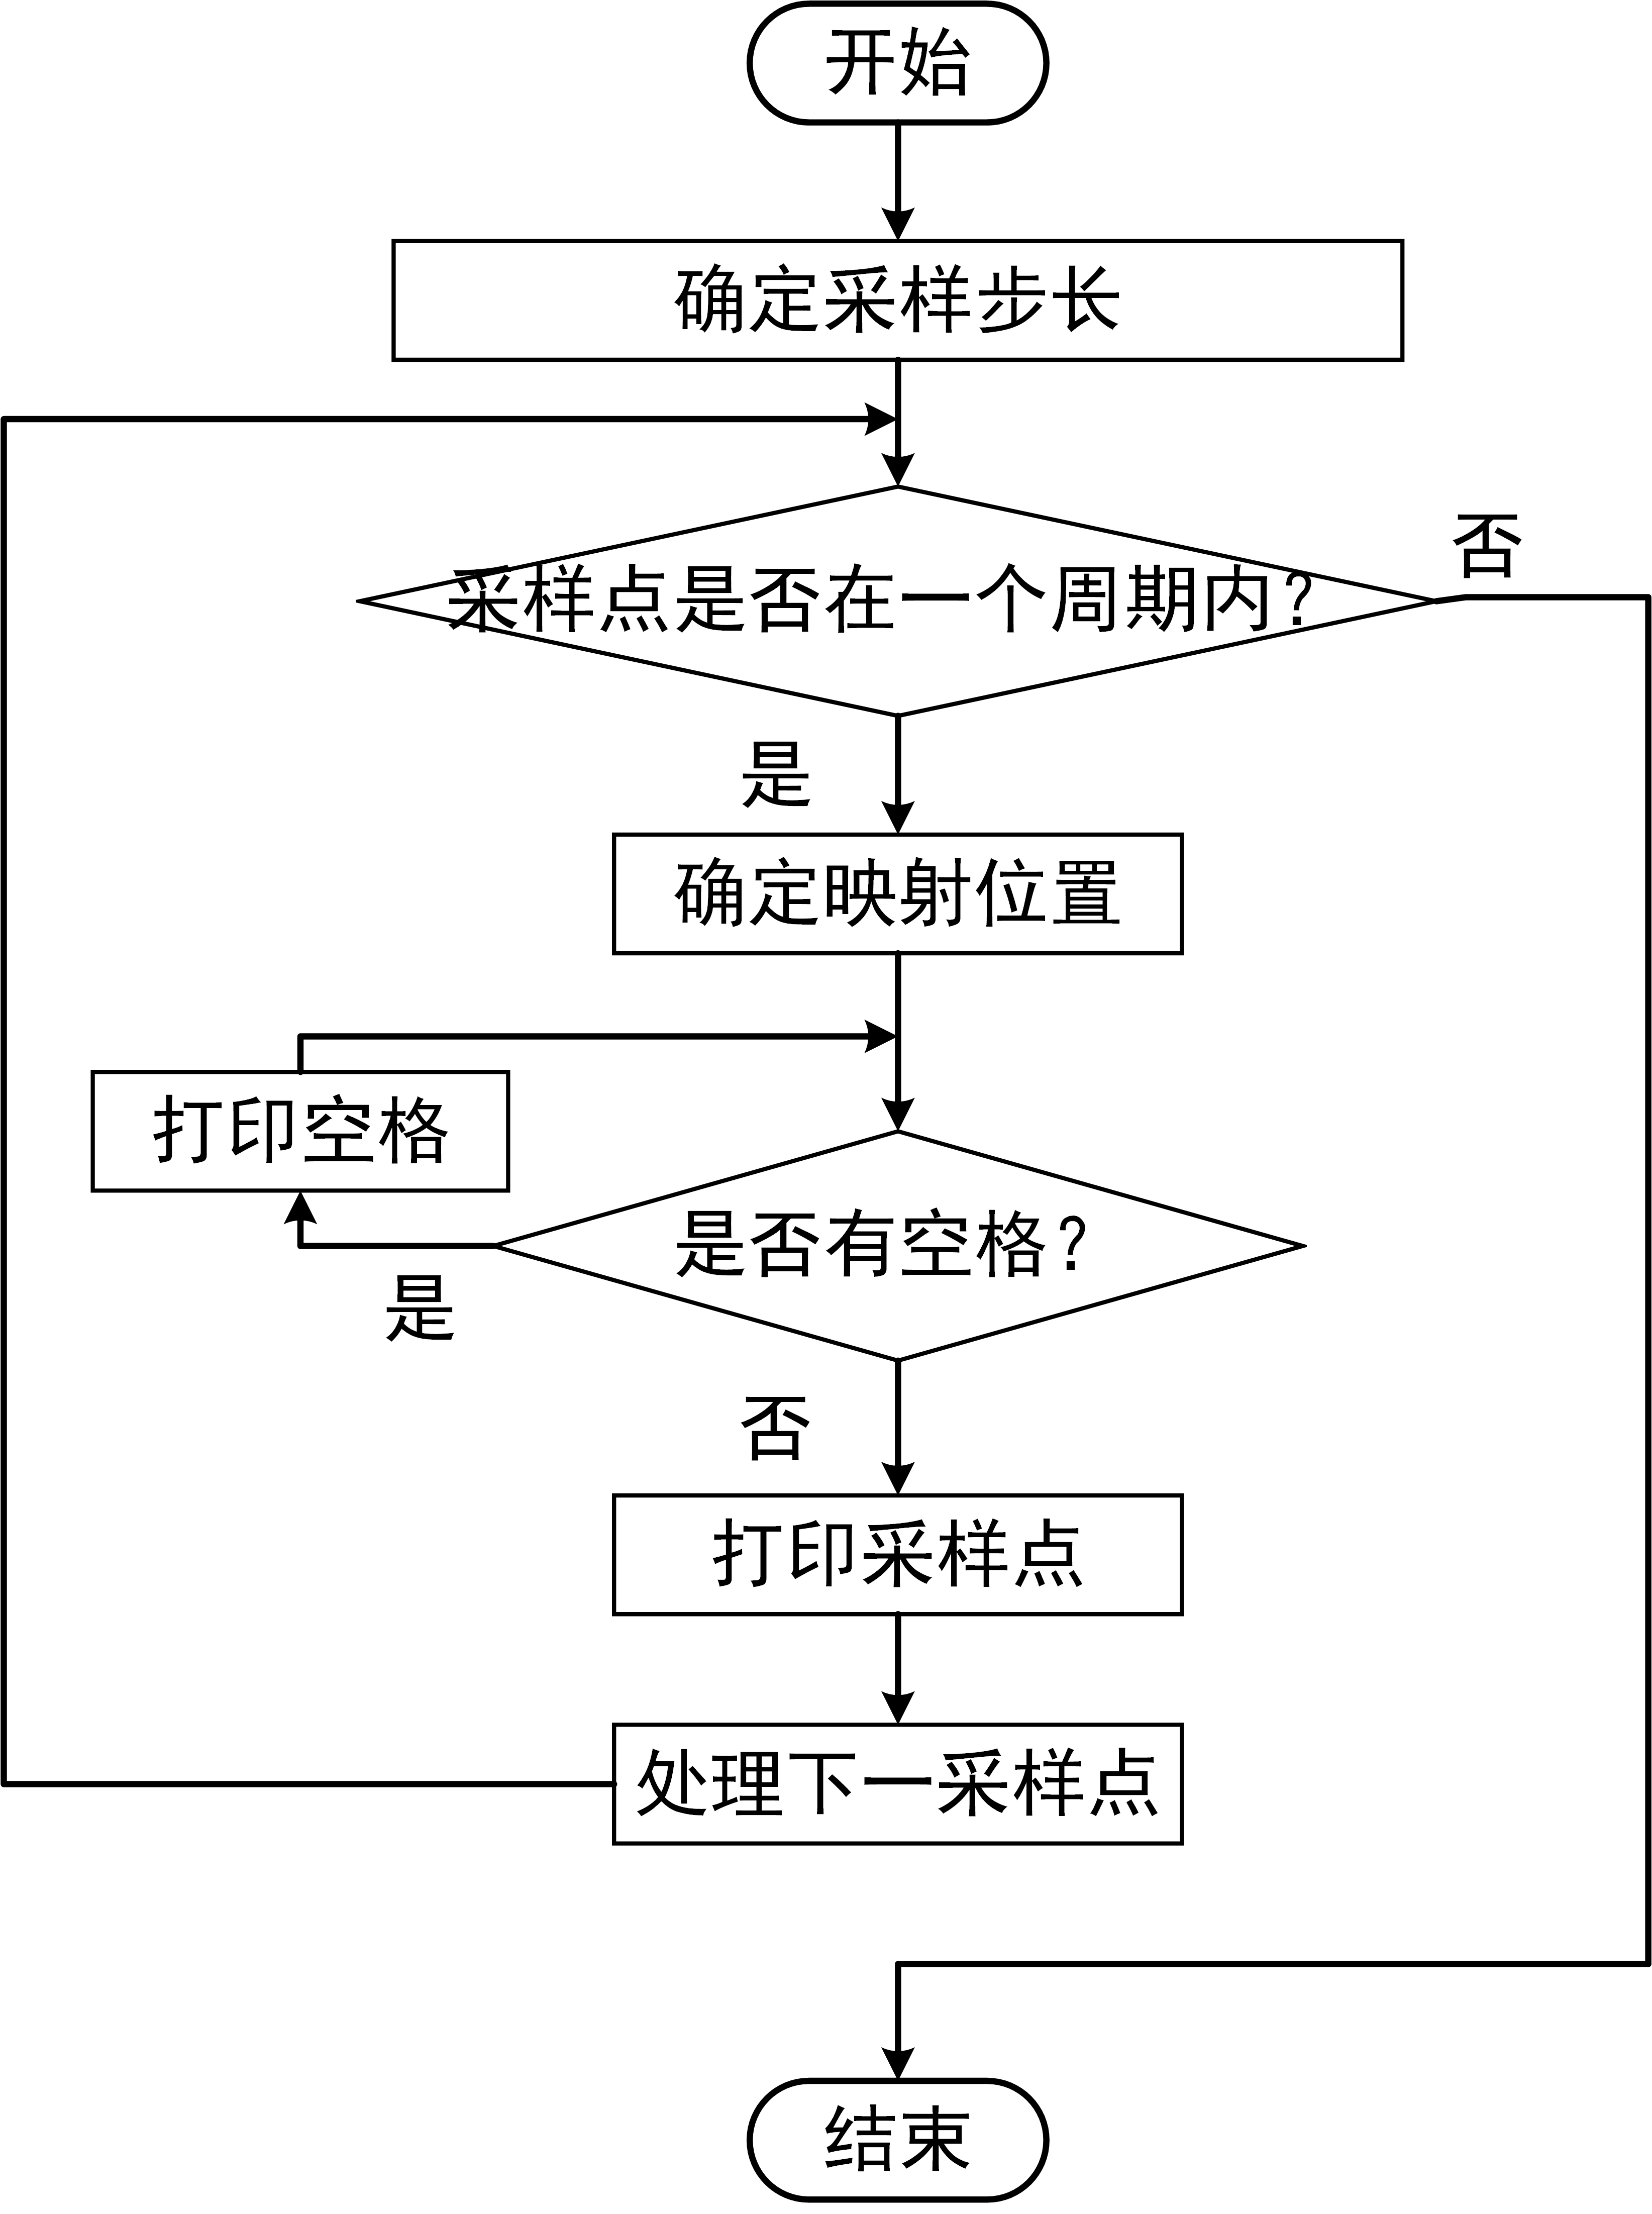
\includegraphics[scale=0.23]{example3_7.png}
				% \caption{程序主要流程}
				% \label{fig:label}
			\end{figure}
		\end{column}
		\hfill

		\begin{column}[b]{0.48\linewidth}
			\begin{figure}[ht]
				\centering
				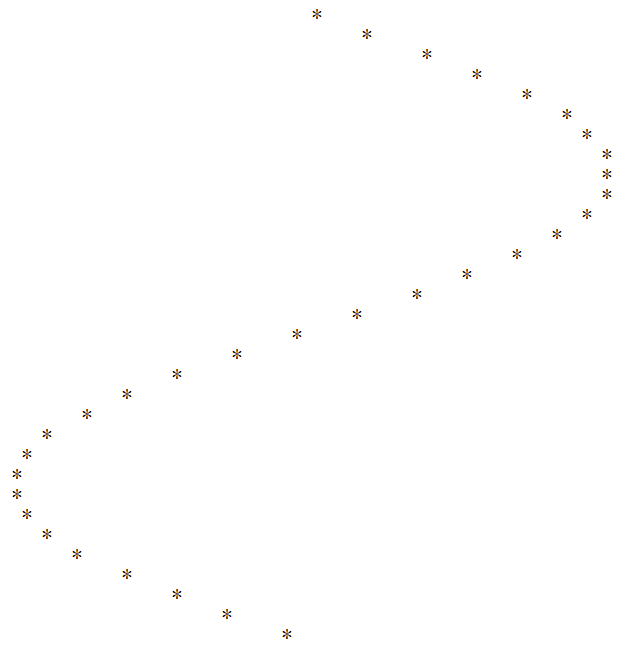
\includegraphics[scale=0.17]{Fig3-2.png}
				% \caption{\texttt{sin(x)曲线}}
				% \label{fig:label}
			\end{figure}
		\end{column}
	\end{columns}
\end{frame}

\begin{frame}[fragile]
	\frametitle{3.5 嵌套结构和应用实例}
	% \framesubtitle{——break 语句}
	\begin{exampleblock}{代码清单3.9,例3.7:}
		\begin{columns}
			\begin{column}{0.06\linewidth}
			\end{column}
			\begin{column}{0.94\textwidth}
				\begin{lstlisting}[numbers=left,numberstyle=\small,basicstyle=\small\ttfamily]
using namespace std;
int main() {
    double step = 0.2;                      //x增加的步长
    double x = 0;                           //x从0开始
    while (x < 6.28) {                      //画一个周期的曲线
        int val = 30*(sin(x)+1);            //计算sin(x)左侧的空格数
        for (int i = 0; i < val; ++i){      //画出所有空格
            cout << " ";
        }
        cout << "*" << endl;                //在相应的位置打印*
        x += step;                          //处理下一个x
    }
    return 0;
}
    \end{lstlisting}\ttfamily
			\end{column}
		\end{columns}
	\end{exampleblock}
\end{frame}


\begin{frame}[fragile]
	\frametitle{3.5 嵌套结构和应用实例}
	% \framesubtitle{——break 语句}
	
	\begin{columns}
		\begin{column}{0.4\textwidth}
\begin{exampleblock}{例3.8:石头剪刀布游戏}
		% \begin{columns}
		%     \begin{column}{0.4\textwidth}
		\ttfamily{玩家和电脑出法相减结果如右图所示。}
			%\alert{提示}:程序主要流程如左图所示}
	\end{exampleblock}
			\begin{figure}[ht]
				\centering
				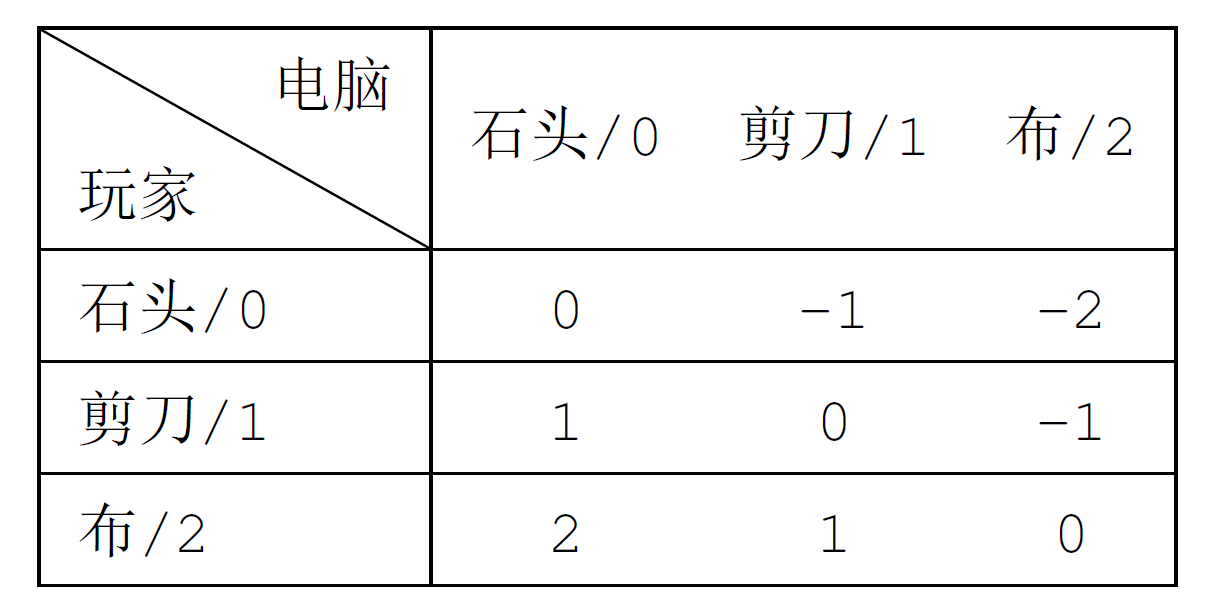
\includegraphics[scale=0.19]{Fig3-3.png}
				% \caption{\texttt{程序主要流程}}
				% \label{fig:label}
			\end{figure}
		\end{column}
		\begin{column}<2->{0.55\textwidth}
			\begin{figure}[ht]
				\centering
                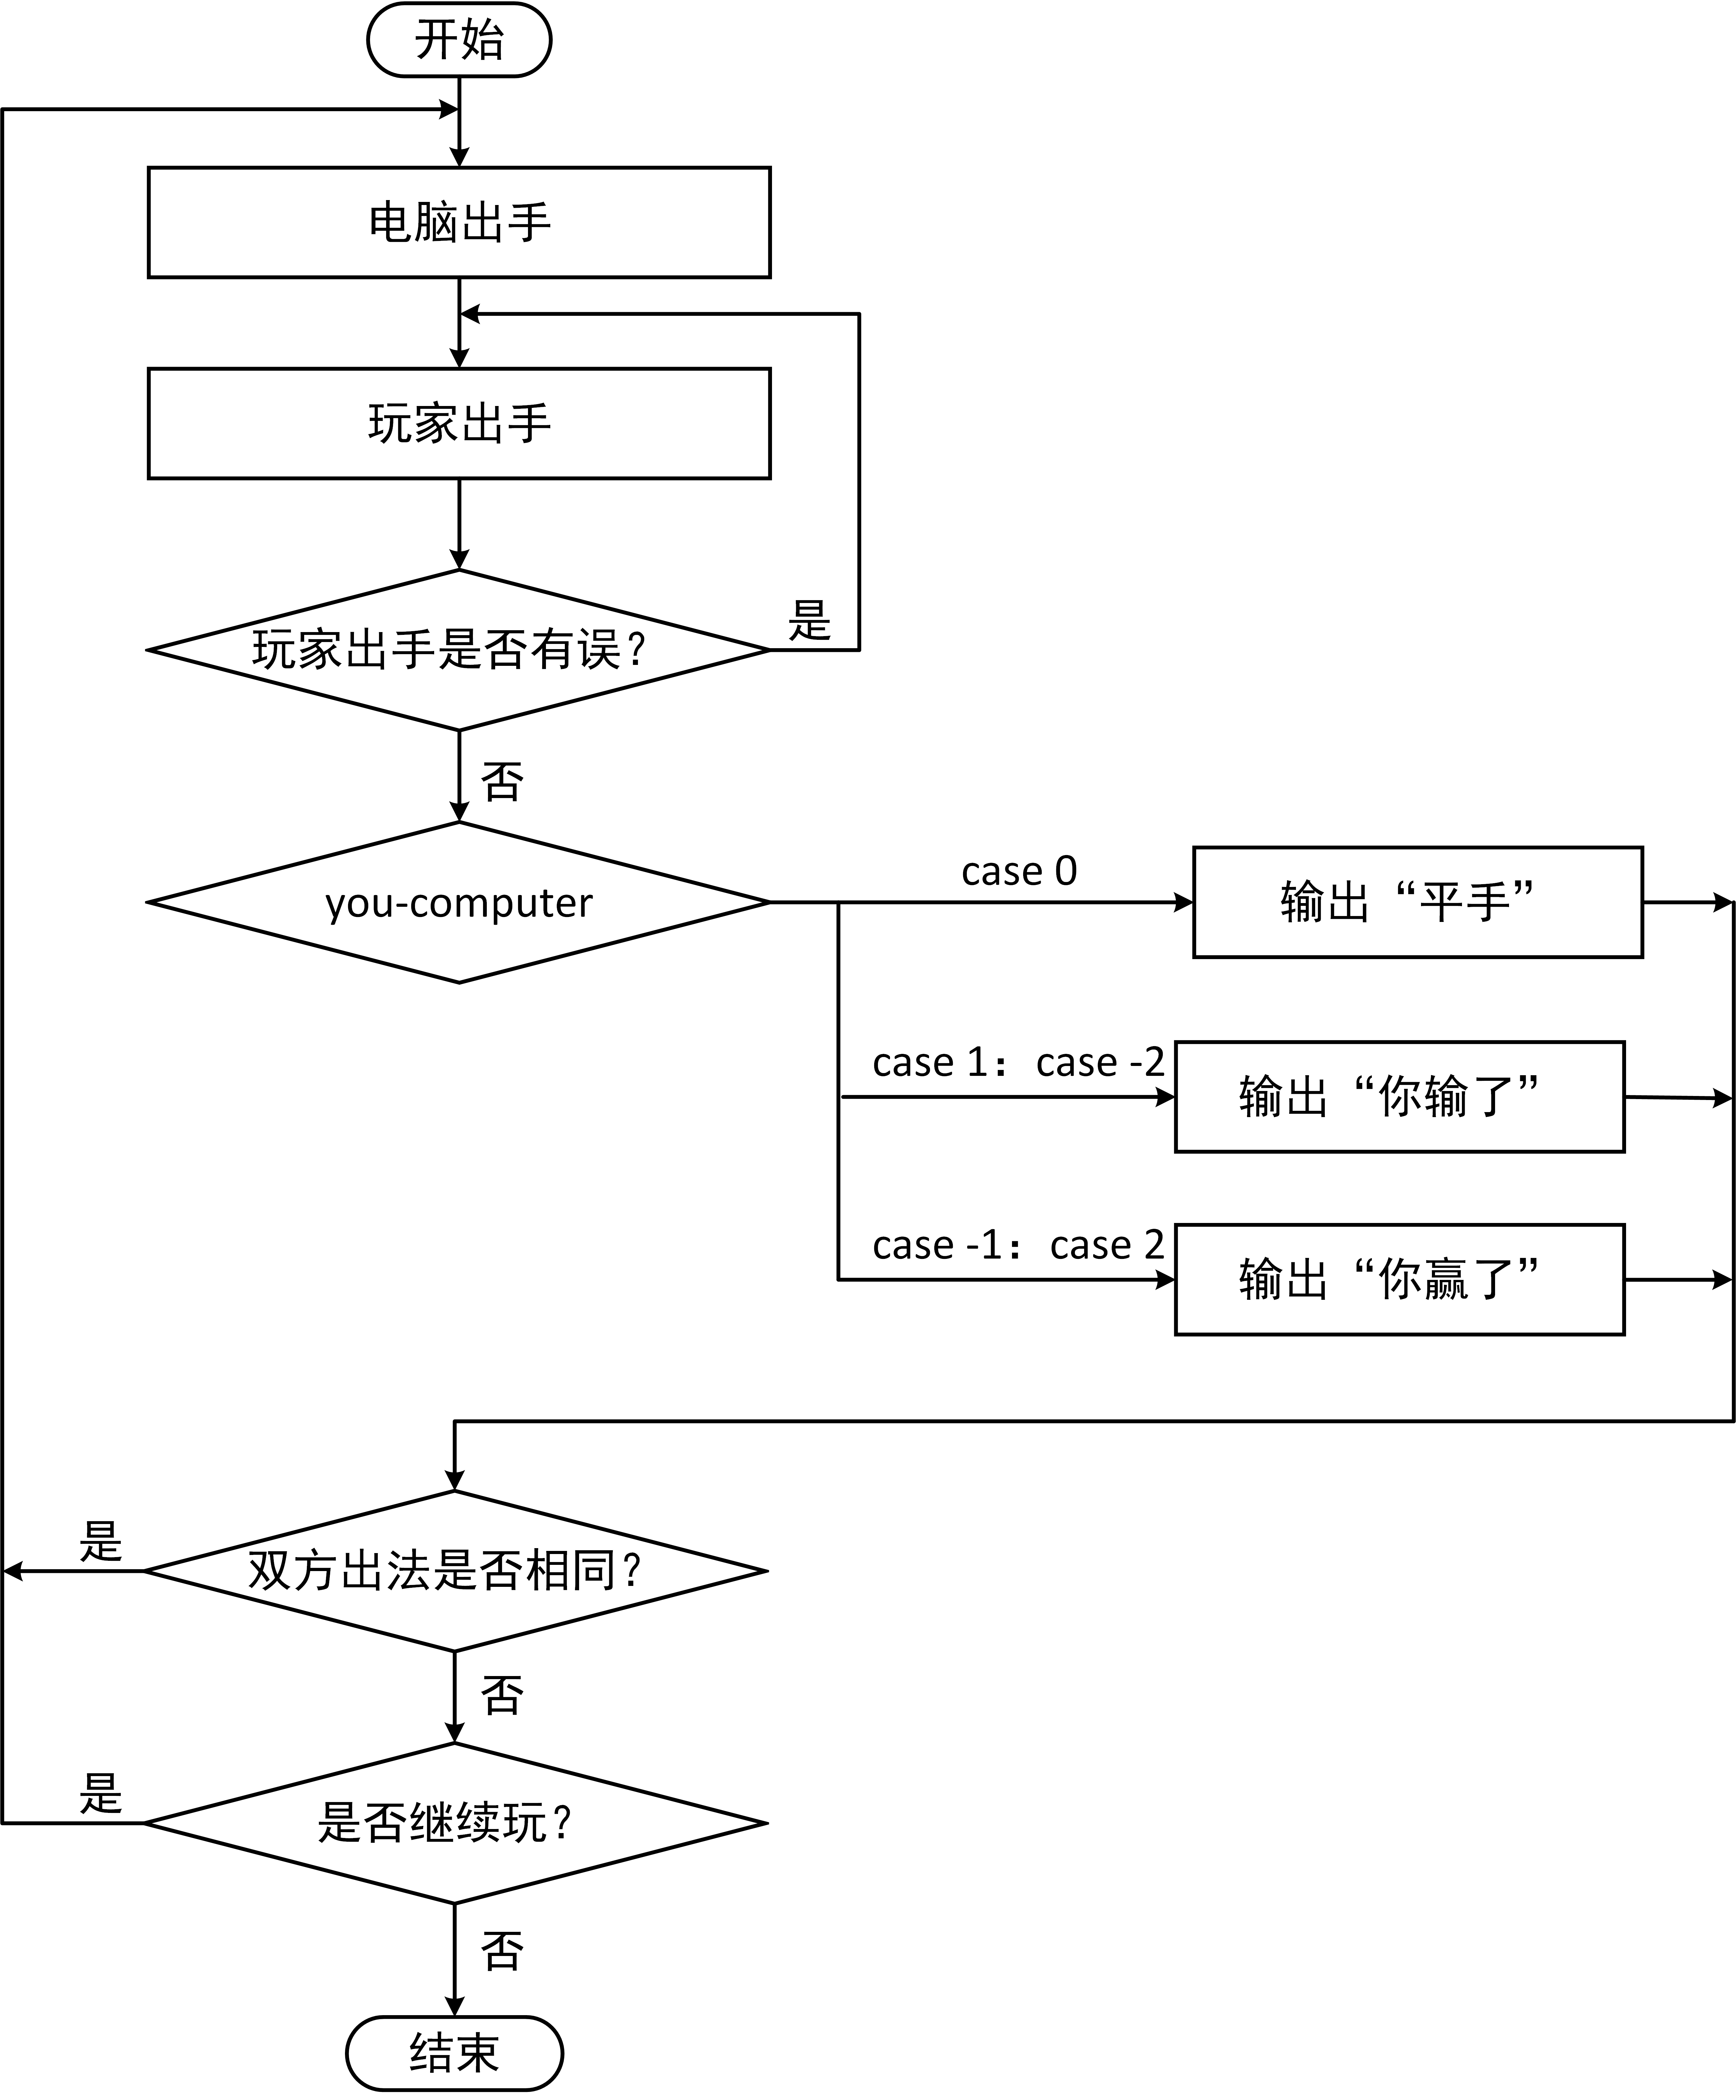
\includegraphics[scale=0.26]{example3_8.png}
				% \caption{\texttt{玩家和电脑出法编号相减结果}}
				% \label{fig:label}
			\end{figure}
		\end{column}
	\end{columns}
\end{frame}

\begin{frame}[fragile]
	\frametitle{3.5 嵌套结构和应用实例}
	% \framesubtitle{——break 语句}
	\begin{exampleblock}{代码清单3.10,例3.8:}
		\begin{columns}
			\begin{column}{0.06\linewidth}
			\end{column}
			\begin{column}{0.94\textwidth}
\vspace{-5mm}
				\begin{lstlisting}[numbers=left,numberstyle=\small,basicstyle=\small\ttfamily]
int main() {
    srand(time(0));
    while (1) {
        int computer, you;
        do {
            computer = rand() % 3;
            do {
                cout << "请出手, 0(石头), 1(剪刀), 2(布):";
                cin >> you;
            } while (you < 0 || you > 2);//如果输入有误,从新输入
            switch (you - computer) {
            case 0:
                cout << "平手" << endl;
                break;
    \end{lstlisting}\ttfamily
			\end{column}
		\end{columns}
	\end{exampleblock}
\end{frame}

\begin{frame}[fragile]
	\frametitle{3.5 嵌套结构和应用实例}
	% \framesubtitle{——break 语句}
	\begin{exampleblock}{代码清单3.10,例3.8:}
		\begin{columns}
			\begin{column}{0.06\linewidth}
			\end{column}
\vspace{-5mm}
			\begin{column}{0.94\textwidth}
\vspace{-3mm}
				\begin{lstlisting}[numbers=left,numberstyle=\small,firstnumber=15,basicstyle=\small\ttfamily]
            case 1: case -2:
                cout << "你输了!" << endl;
                break;
            case -1: case 2:
                cout << "你赢了!" << endl;
            }
        } while (computer == you);//双方出法相同,继续出
        cout << "还要玩吗?Y/N:";
        char play;
        cin >> play;
        if (play == 'N' || play == 'n') break;
    }
    return 0;
}
    \end{lstlisting}
    \onslide<2->{如何让电脑更聪明?提示:尝试人工智能-\alert{强化学习}方法}
			\end{column}
		\end{columns}
	\end{exampleblock}
\end{frame}


\begin{frame}[fragile]
	\frametitle{3.5 嵌套结构和应用实例}
	% \framesubtitle{——break 语句}
	\begin{exampleblock}{例3.9:}
		\ttfamily{公元前五世纪,我国古代数学家张丘建在《算经》一书中提出了(百钱百鸡):鸡翁一值钱五,鸡母一值钱三,鸡雏三值钱一。百钱买百鸡,问鸡翁、鸡母、鸡雏各几何?\\
			\alert{提示}:穷举法:对可能是解的众多候选解按某种顺序进行逐一列举和检验,从中找出符合要求的解。本例穷举示意图如下图所示。}
	\end{exampleblock}
	\begin{center}
		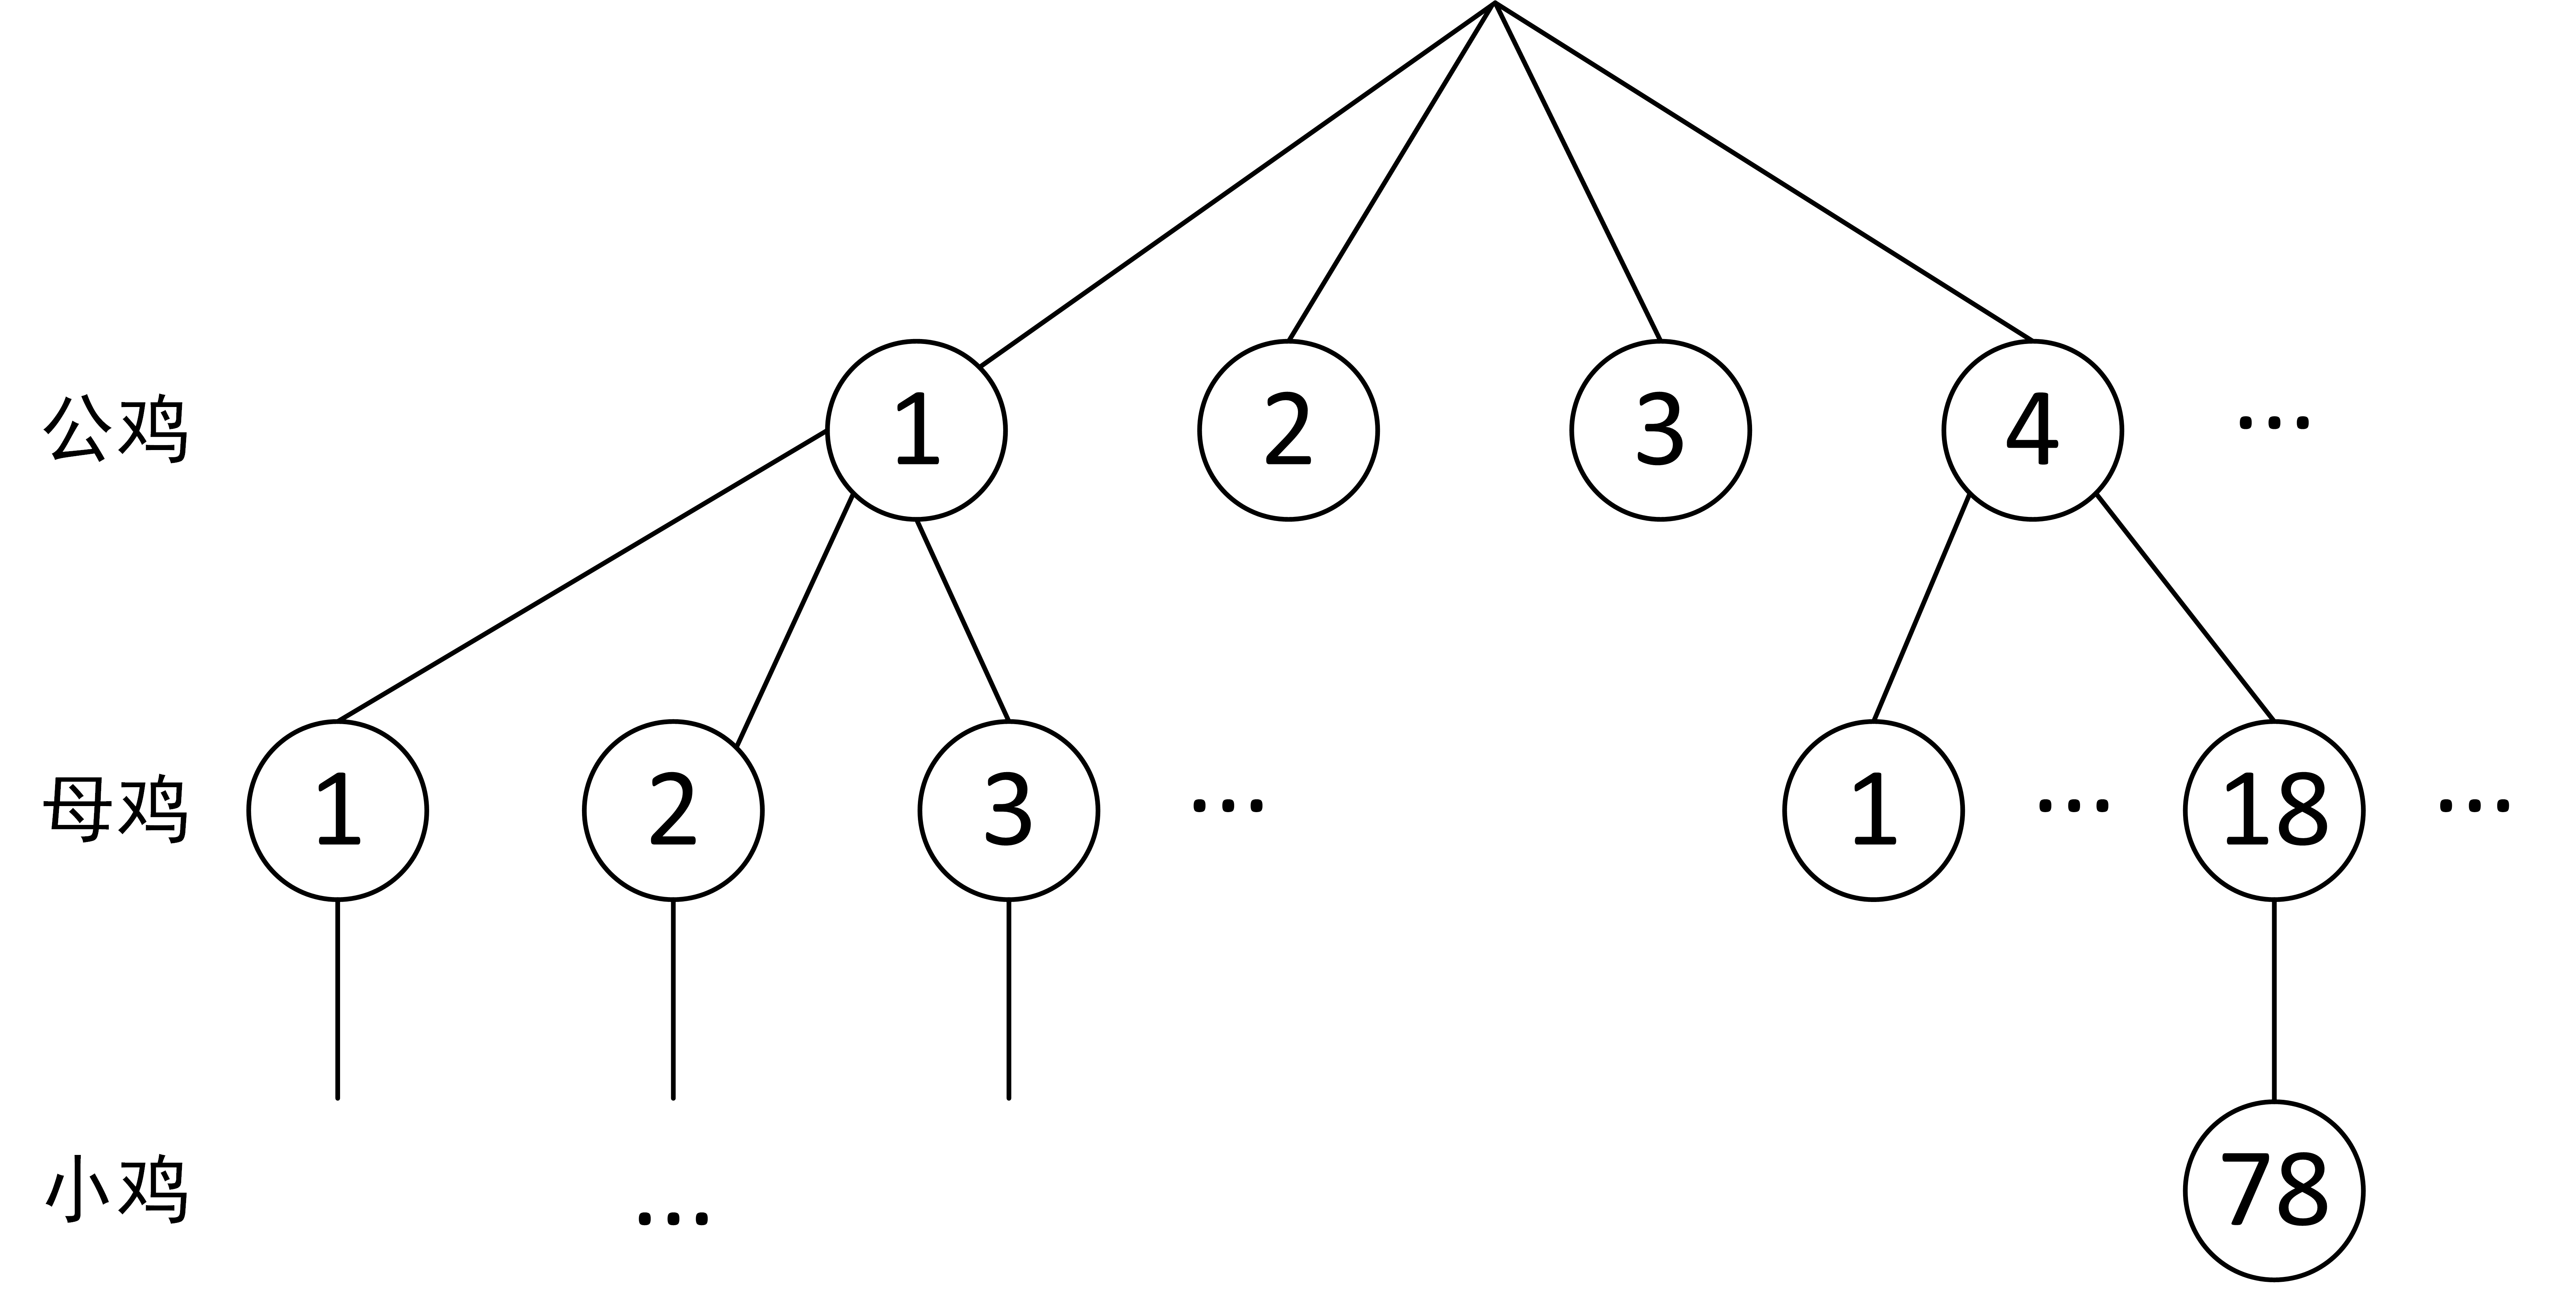
\includegraphics[scale=0.28]{example3_9.png}\\
		\ttfamily 上图中公鸡、母鸡、小鸡数目分别为:4、18、78是一种符合要求的结果
	\end{center}
\end{frame}

\begin{frame}[fragile]
	\frametitle{3.5 嵌套结构和应用实例}
	% \framesubtitle{——break 语句}
	\begin{exampleblock}{代码清单3.11,例3.9:}
		\begin{columns}
			\begin{column}{0.06\linewidth}
			\end{column}
			\begin{column}{0.94\textwidth}\vspace{-3mm}
				\begin{lstlisting}[numbers=left,numberstyle=\small,basicstyle=\small\ttfamily]
#include <iostream>
using namespace std;
int main() {
    int max_rst = 100 / 5, max_hen = 100 / 3;   //公鸡、母鸡最大数目
    for (int i = 0; i < max_rst; ++i) {
        for (int j = 0; j < max_hen; ++j) {
            int k = 100 - i - j;                //小鸡数目
            if (k % 3) continue;    //跳过不能被3整除的数,执行流程跳转到++j
            if (5 * i + 3 * j + k / 3 == 100) {
                cout<<"公鸡:"<<i<<" 母鸡:"<<j<<" 小鸡:"<<k<<endl;
            }
        }
    }
    return 0;
}
    \end{lstlisting}\ttfamily
			\end{column}
		\end{columns}
	\end{exampleblock}
\end{frame}

\begin{frame}[fragile]
	\frametitle{3.5 嵌套结构和应用实例}
	% \framesubtitle{——break 语句}
	\begin{exampleblock}{}
		\ttfamily 输出:\\
		公鸡:0 母鸡:25 小鸡:75\\
		公鸡:4 母鸡:18 小鸡:78\\
		公鸡:8 母鸡:11 小鸡:81\\
		公鸡:12 母鸡:4 小鸡:84\\
	\end{exampleblock}
\end{frame}

%---------------------------------------------------------------------------------------------
\begin{frame}[fragile]{课后作业}
\begin{columns}[t]
\column{0.8\textwidth}
\begin{block}{作业本}
 \begin{enumerate}
   \item 习题3.5、3.6和3.13
 \end{enumerate}
\end{block}

\begin{block}{上机练习}
 \begin{enumerate}
   \item 实验指导书:第三章
 \end{enumerate}
\end{block}
\end{columns}
\end{frame}


\begin{frame}[fragile]
	\frametitle{~~}
	\begin{center}
		\huge{本章结束}
	\end{center}
\end{frame}

\end{document}
